\documentclass{article}
\usepackage[brazil]{babel}

\usepackage[a4paper,top=2cm,bottom=2cm,left=3cm,right=3cm,marginparwidth=1.75cm]{geometry}
% Useful packages
\usepackage{amsmath}
\usepackage{graphicx}
\usepackage[colorlinks=true, allcolors=blue]{hyperref}
\usepackage{minted}
\usepackage{float}
\usepackage{soul}

\title{Relatório Anual PIBIC 10}
\author{Daniel Brito dos Santos}

\begin{document}
\begin{titlepage}
\begin{center}
\large
\textbf{PROGRAMA INSTITUCIONAL DE BOLSAS DE INICIA\c{C}\~{A}O CIENTIF\'{I}CA E TECNOL\'{O}GICA\\\vspace{0,5cm}
UNIVERSIDADE ESTADUAL DO NORTE FLUMINENSE DARCY RIBEIRO\\
}
\textit{Centro CCT \\
Labotat\'{o}rio LCMAT\\
\vspace{1cm}
Relat\'{o}rio do per\'{\i}odo: Março 2021 - Janeiro 2022}\\
\vspace{1,5cm}
\textbf{Relat\'{o}rio Anual PIBIC-10}\\\vspace{5cm}
\end{center}
\textbf{Bolsista}: Daniel Brito dos Santos\\
\textbf{Matricula}: 00119110393\\
\textbf{Orientadora}: Prof. Dra. Annabell Del Real Tamariz  \\
\textbf{Curso}: Bacharelado em Ci\^{e}ncia da Computa\c{c}\~{a}o\\
\vspace{3cm}
\begin{center}
\textbf{Titulo do Projeto}: Project-driven \textit{Data Science}: Aprendendo e Mapeando\\
\textbf{T\'{\i}tulo do Plano de Trabalho}: Ponta do Iceberg: primeiros passos na Ciência de dados\\
\textbf{Fonte financiadora:} PIBIC/UENF
\end{center}
\end{titlepage}



\section{Introdução}
Em 1962, John Tukey publicou o artigo "The Future of Data Analysis" na revista científica The Annals of Mathematical Statistics \cite{FoDA}. Sendo o principal veículo para publicações de estatística matematicamente avançada, os outros artigos na revista apresentavam definições, teoremas e provas. Enquanto isso, o artigo de Tukey era basicamente uma confissão pública, explicando porquê ele achava esse tipo de pesquisa restritiva, possivelmente inútil e danosa. \cite{DONOHO}
Para ele, o escopo da pesquisa estatística deveria ser drasticamente ampliado e redirecionado. Nesse sentido, Tukey introduziu o termo "data analysis" para nomear o trabalho dos estatísticos práticos, diferenciando-o da inferência estatística formal. 
Assim, seu argumento central é de que a estatística é parte de uma entidade maior, entidade esta que não seria apenas um braço da matemática, mas sim uma nova ciência. Uma ciência definida pelo problema onipresente que ela busca resolver ao invés de se definir pelo seu objeto concreto \cite{DONOHO}.

Não é surpreendente que a resposta ao seu artigo tenha sido tímida, e hostíl.\cite{DONOHO} No próprio artigo, Tukey admite que extendeu o termo "data analysis" muito além de sua filologia, a tal ponto de na verdade englobar toda a estatística e ainda mais. Ele admite também que é um campo difícil, tanto a sua formalização quanto sua prática, e portanto deve se adaptar ao que as pessoas podem e precisam fazer com dados. Em suas palavras \cite{FoDA}:
\begin{quote}
Assim como biologia é mais complexa que física, ciência do comportamento é mais complexa que ambas, é provável que os problemas gerais de \textit{data analysis} sejam mais complexos que os problemas de cada uma dessas três disciplinas. 
De modo que é pedir demais esperar uma orientação próxima e eficaz de uma estrutura altamente formalizada, agora ou em um futuro próximo. 
\end{quote}

Entretanto, o desafio que essa área apresenta é proporcional ao seu potencial disruptivo, como ficaria claro ao longo das décadas seguintes. \cite{DONOHO} argumenta que "em última instância, o que tornou essa atividade chamada 'data analysis' concreta foi código, e não palavras". De modo que a partir do compartilhamento dos scripts computacionais para análise de dados, principalmente potencializado pelo que o autor chama de \textit{Common Task Framework} (CTF), e todo o contexto de profusão de dados, crescimento do poder computacional e da mudança de paradigma que ela representou, o que atualmente chamamos de ciência de dados se consolidou como um dos principais campos de pesquisa e trabalho da atualidade. \cite{DSmktshare}

As CTFs foram as competições abertas nas quais grupos diferentes poderiam submeter seus scripts para resolver um desafio de dados, de modo a premiar e implementar as melhores soluções. Esse fenômeno foi resultado direto da observação de Tukey sobre a mudança de paradigma de otimizar o valor gerado no mundo real ao invés da elegância matemática. 

Esse foco na geração de valor torna essa nova ciência extremamente relevante no contexto das necessidades empresariais e sociais que temos: aumentar eficiência, entregar produtos melhores, criar soluções relevantes, analisar impacto de políticas, organizar a torrente continua de informação coletada o tempo inteiro. 

Logo, esse enfoque trouxe muitos resultados, por exemplo o sucesso de algumas das empresas mais valiosas do mundo como a Amazon\footnote{www.amazon.com}, Google\footnote{google.com}, Facebok\footnote{facebook.com} e Netflix\footnote{netflix.com}, nas quais o seu produto é fruto direto de seu processamento de dados \cite{DATAHUNGRY}. Tanto que nelas foi inaugurado o cargo "cientista de dados". Que logo foi denominada "a profissão mais sexy do século XXI" pela revista \href{https://hbr.org/2012/10/data-scientist-the-sexiest-job-of-the-21st-century}{Harvard Bussiness Review}\footnote{hbr.org/2012/10/data-scientist-the-sexiest-job-of-the-21st-century}.

Nesse contexto se consolidou a Ciência de Dados (DS) que pode ser definida como o campo de conhecimento fundamentalmente interdisciplinar; responsável por aplicar, organizar e expandir o conjunto de ferramentas, técnicas e conceitos necessários no processo de transformação de dados brutos em informações relevantes. 
Normalmente, utiliza-se modelos preditivos para modelar matematicamente relações entre variáveis de entrada de modo que permita inferir novos valores a partir de novas variáveis de entrada.  

Entretanto, considerando a amplitude de sua “caixa de ferramentas”, a necessidade de repertório para aplicá-las, a diversidade dos problemas abordados e a velocidade com que todo o campo se desenvolve, a formação de cientista de dados é um desafio inerente à própria natureza desse campo,\cite{BATON,DONOHO}.

Assim, nosso projeto se insere como um primeiro passo na tentativa de mapear essa nova ciência. Elencar os seus principais conceitos e ferramentas. 
Para tanto, revisamos a diversa literatura disponível tanto em livros quanto artigos e até mesmo sites interativos. Bem como executamos um projeto representativo para exemplificar e consolidar as principais técnicas e ferramentas utilizadas em cada etapa de um projeto de dados. 

O projeto selecionado foi o Projeto Titanic, disponível na plataforma Kaggle\footnote{www.kaggle.com/c/titanic}.
Essa plataforma é um dos principais recursos para a prática e aprendizado da ciência de dados. Pois nela encontramos fórums de discussão, minicursos, e principalmente competições de dados semelhantes aos CTFs mencionados por \cite{DONOHO}, onde é apresentado um problema e um conjunto de dados, de modo que cada usuário pode construir e submeter a sua solução, que será automaticamente avaliada e \textit{rankeada} junto às outras soluções submetidas. 

O grande impacto que essa estrutura oferece é a possibilidade de competição colaborativa, pois ao mesmo tempo que cada um desenvolve a sua rotina de análise, os notebooks podem ser publicados e discutidos, e dessa maneira muitos problemas inéditos foram resolvidos \cite{KAGGLE_OPPORTUNITY,KAGGLEgraham2015,KAGGLEiglovikov2017,KAGGLEnarayanan2011,KAGGLEpuurula2014,KAGGLEtaieb2014,KAGGLEyang2018}. 

Tais soluções são construídas em notebooks, análogos aos Jupyter Notebooks, ou seja células interativas que podem conter código ou texto e que, segundo \cite{BATON}, se tornaram o principal ambiente de desenvolvimento dos cientistas de dados. Os notebooks do Kaggle ainda oferecem processamento e armazenamento online gratuitos.

Finalmente, selecionamos o Titanic por ser a competição sugerida como introdução tanto à plataforma, quanto a projetos de dados. 

\section{Etapas propostas no plano de trabalho}
O plano de trabalho original consistiu em desenvolver o Projeto Titanic de acordo com as etapas canônicas de um projeto de dados. Desse modo, em cada passo executamos o projeto, e utilizamos seu contexto para o estudo direcionado dos conceitos e ferramentas necessárias àquela etapa. Foram elas:
\begin{enumerate}
\item Bases gerais
\item Definição de problema
\item Obtenção de dados
\item Data Analysis
\item Aprendizado de Máquina ou Machine Learning
\item Data Vizualization
\item Deployment 
\item Elaboração do relatório final.
\end{enumerate}

Executamos todas as etapas do projeto. Identificamos, entretanto, que as etapas de Aprendizado de Máquina, Data Vizualization e Deployment trazem consigo uma complexidade maior em função de serem áreas autárquicas com seus próprios corpus de conhecimentos. O que inspira futuros desenvolvimentos para atingirmos o objetivo principal de cartografar o campo da ciência de dados. 

\section{Objetivos}
Nosso objetivo nesse primeiro ano foi mapear e delinear os contornos do atual campo conhecido como Ciência de Dados. Explicitar a sua definição, seus principais métodos, conceitos e ferramentas. Bem como consolidar e exemplificar o aprendizado por meio da execução de um projeto representativo. 

\section{Metodologia}
Utilizamos uma metodologia diversificada para abordar os diferentes aspectos do projeto. De modo que o separamos em subprojetos de acordo com as etapas canônicas de um projeto de dados, principalmente inspiradas nos cinco passos definidos por \cite{PRINCIPLES}: 

\begin{itemize}
\item Construir uma pergunta interessante
\item Obter os dados
\item Explorar os dados
\item Modelar os dados
\item Comunicar e visualizar os resultados
\end{itemize}

Assim, a cada etapa, buscamos o ferramental necessário e executamos os passos correspondentes no projeto Titanic. 

Além dessa pesquisa teórica, o bolsista também se familiarizou com a plataforma Kaggle. Especialmente no que diz respeito ao projeto Titanic por meio do estudo da \href{https://www.kaggle.com/c/titanic}{página do projeto}\footnote{https://www.kaggle.com/c/titanic}, tendo em vista compreende-lo para aplicar o que foi estudado teoricamente sobre a estruturação e execução de um projeto de dados.


\subsection{Bases Gerais}\label{Bases Gerais}
O primeiro dos subprojetos foi o estudo da área em si. Iniciamos o processo de familiarização a partir da leitura dos livros \cite{PRINCIPLES} e \cite{DOING}. 
Posteriormente, percebemos que há um importante debate quanto a definição de ciência de dados como um campo. Portanto, entendemos necessário buscar referencial teórico na literatura para definirmos Ciência de Dados, de modo a delimitarmos o escopo de sua prática e teoria, modelo de trabalho e pressupostos.

Nesse sentido pesquisamos o termo "\textit{Data Science}" na plataforma de busca "Google Scholar"\footnote{scholar.google.com}, filtramos apenas os artigos do tipo revisão. Percorremos as primeiras 100 páginas de resultados avaliando manualmente seus títulos e resumos (\textit{abstracts}). Assim, selecionamos os artigos que têm por objeto a caracterização rigorosa da Ciência de Dados, seu campo, teoria e prática. Uma vez selecionados, os artigos foram lidos sistematicamente de modo a construir a partir dos mesmos um panorama dessa área. 

\subsection{Definição de problemas de dados}
Nessa etapa voltamos aos livros \cite{DATAPYTHON}, \cite{PRINCIPLES} e principalmente ao modelo de trabalho definido por \cite{BATON}, encontrado como resultado da pesquisa na etapa anterior (seção \ref{Bases Gerais}). De modo a identificar e compreender de forma mais ampla as ferramentas e preocupações que cientistas de dados devem ter ao iniciar um projeto. 

\subsection{Obtenção de Dados}
Iniciamos essa etapa estudando a obtenção de dados, usando o livro \cite{DATAPYTHON}, e seguindo as diretrizes do modelo \cite{BATON}.  Nesse contexto, também buscamos elencar os principais recursos para aprendizagem da linguagem SQL \cite{chamberlin1974sequel}. Isto porque bancos de dados relacionais são uma das mais importantes fontes de dados para um cientista de dados, portanto dominar a sua língua franca é essencial para um profissional dos dados \cite{SCRATCH,DATAPYTHON}. Não utilizamos SQL no Titanic devido ao fato de ser um projeto introdutório no qual os dados já foram fornecidos no formato de uma tabela simples e organizada, portanto não foi necessário utilizarmos bancos de dados. 

Nesse sentido, para obtermos os dados para o projeto Titanic utilizamos as instruções do Kaggle bem como a documentação oficial da biblioteca Pandas\footnote{pandas.pydata.org}. Essa biblioteca é a principal ferramenta para obtenção e análise de dados em Python. Ela oferece estruturas de dados especiais para trabalhar com conjunto de dados, sendo o DataFrame a sua principal estrutura. Com ela podemos repartir, agrupar, ler diversos tipos de arquivo, criar visualizações rápidas, aplicar funções a colunas, dentre várias outras funcionalidades.
Na sequencia apresentam-se os passos seguidos:
\begin{enumerate}
    \item Criar um novo notebook para o projeto, em sua \href{https://www.kaggle.com/c/titanic}{página principal}\footnote{https://www.kaggle.com/c/titanic} selecionamos a aba \textsc{code} e clicamos no botão \textsc{new notebook}, vide Figura \ref{create_notebook}.
    \begin{figure}[H]
     \centering
     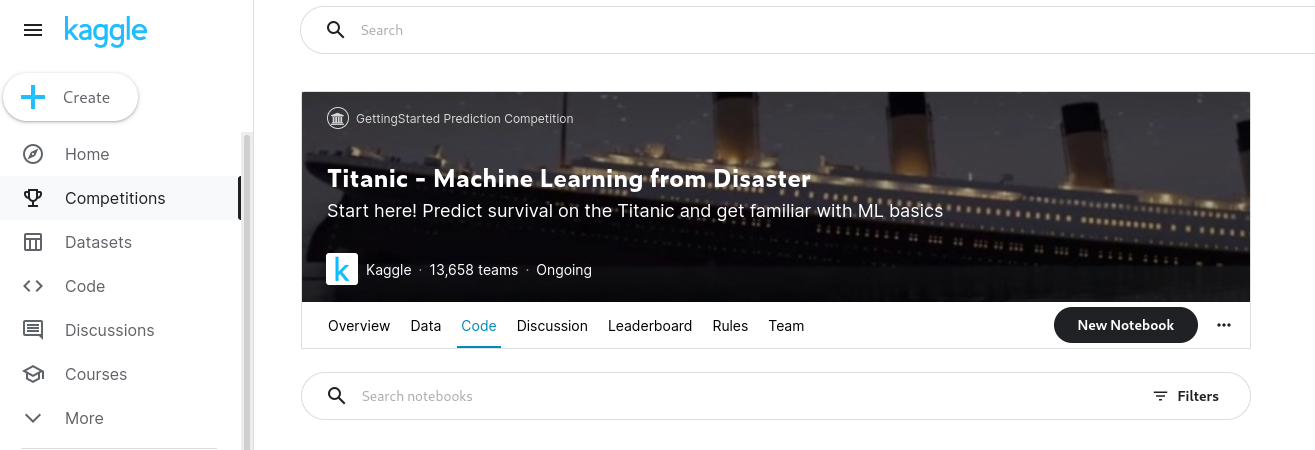
\includegraphics[width=\textwidth]{Figures/create_notebook.png}
     \caption{\label{create_notebook}Criação de um novo notebook.}
    \end{figure}
    
    \item Como se mostra na Figura \ref{new_notebook}, nosso novo notebook já tem o código para a listar os arquivos disponíveis, bem para carregar as bibliotecas normalmente utilizadas nesse contexto, dentre elas utilizaremos a Pandas. A outra biblioteca carregada é a Numpy, é a principal ferramenta para computação numérica e álgebra linear em Python, não será utilizada diretamente nesse projeto, mas é fundamental em muitas operações numéricas mais complexas.   
    \begin{figure}[H]
     \centering
     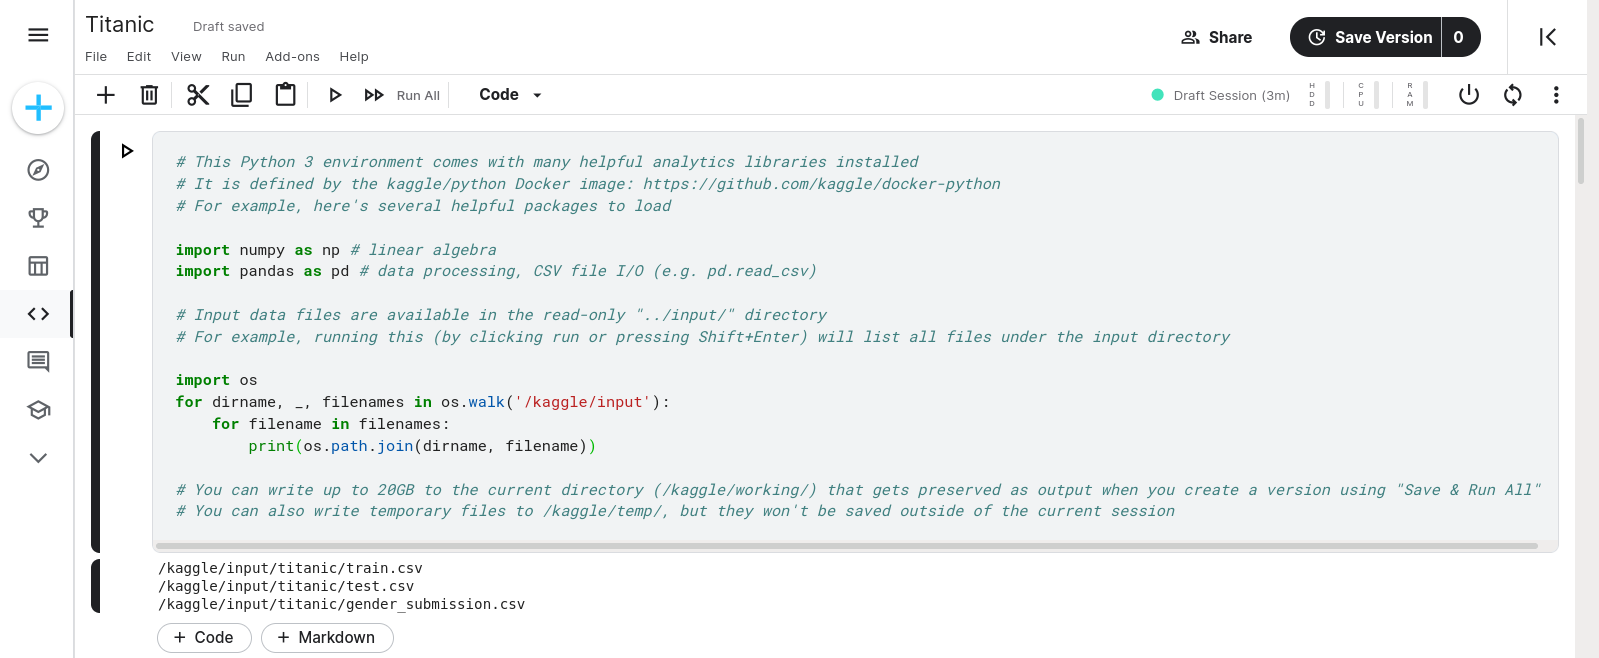
\includegraphics[width=\textwidth]{Figures/kaggle_new_notebook.png}
     \caption{\label{new_notebook}Notebook criado.}
    \end{figure}
    
    \item Assim, utilizamos a função \textsc{read\_csv()} da biblioteca Pandas (importada com o "apelido" de "pd", vide Figura \ref{new_notebook}), com o endereço do arquivo desejado.
    Assim, carregamos na memória e armazenamos em variáveis os três arquivos disponíveis no Titanic: 
    \begin{itemize}
        \item train.csv, arquivo principal que utilizaremos para analisar e processar.
        \item test.csv, arquivo que será utilizado para gerar nossa solução final que será submetida para avaliação da plataforma Kaggle.
        \item gender\_submmission.csv, arquivo que exemplifica a submissão final à plataforma. Nesse caso gender por exemplificar utilizando o gênero como única variável para determinar a predição. 
    \end{itemize}
    
    
    para carregarmos a tabela de treinamento e a tabela de teste respectivamente na memória, também criamos uma cópia do \textsc{DataFrame} \textsc{train} para a variável \textsc{df}, tendo em vista podermos alterar \textsc{df}, mantendo em memória o \textsc{DataFrame} original "train".
    Apresenta-se, na Figura \ref{read_csv}, os comandos executados para esse fim. 
    
    \begin{figure}[H]
     \centering
     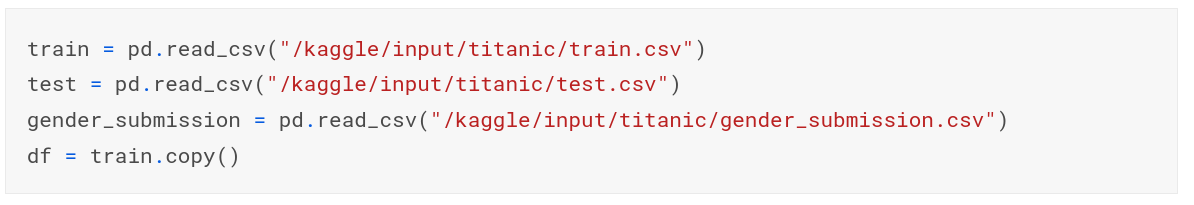
\includegraphics[width=\textwidth]{Figures/read_csv.png}
     \caption{\label{read_csv}Carregamento das tabelas.}
    \end{figure}
\end{enumerate}

\subsection{Data Analysis}\label{Data Analysis}
Nessa etapa, iniciamos construindo um repertório de técnicas e conceitos a partir das ideias de \cite{DATAPYTHON}, \cite{BATON}, e simultaneamente exploramos os dados desenvolvendo a análise do projeto Titanic. Assim como utilizamos o ecossistema construído, aliado aos referenciais teóricos para ganhar fluência no ecossistema da linguagem Python para análise de dados. Isto é, utilizando a biblioteca Pandas para ler arquivos CSV, processar tabelas e transformar dados. 

\subsubsection{Técnicas e conceitos}
\begin{itemize}
\item Utilizamos a função \textsc{.info()} da biblioteca Pandas para nos apresentar um resumo da tabela: lista de suas colunas, quantidades de linha, número de entradas em cada linha. Por exemplo, usando o comando \textsc{df.info()}, obtém-se um resumo da tabela de treinamento \textsc{df}. Maiores detalhes podem ser observados na Figura \ref{df.info} na seção \ref{resultados}.
\item Utilizamos a função \textsc{.describe()} para observarmos o resumo estatístico dos dados, apresentando dados como média, desvio padrão, quartis. 
\item Utilizamos a função \textsc{.map()} para mapear cada entrada da coluna a um dicionário. Desse modo, a função percorre cada entrada de uma determinada coluna e caso seu valor esteja presente como chave do dicionário, a função o substitui pelo valor do dicionário. Assim podemos por exemplo ter uma coluna "Sex" com valores 'male' e 'female' e um dicionário {'male':0,'female':1}, ao aplicar o dicionário na coluna, as strings serão substituídas pelos inteiros correspondentes. Assim podemos fazer análises numéricas dessa coluna também. 
\item Utilizamos a função \textsc{groupby()} para relacionar duas colunas e observar seu comportamento de acordo com a outra. Por exemplo, podemos observar a média da idade dos sobreviventes, e comparar com a média de idade dos que não sobreviveram. Nesse caso agrupamos todas as variáveis numéricas de acordo com a sobrevivência, de modo que temos a média de cada coluna em cada destino.
\item \textsc{.hist()} nos apresenta o histograma da coluna selecionada. Como parâmetros opcionais utilizamos o \textsc{bins=} para determinar quantas barras serão utilizadas, \textsc{sharex=True} para ambos os histogramas compartilharem o eixo x, \textsc{sharey=False} para que a escala de y possa ser de acordo com cada histograma, assim podemos ver a diferença percentual e não apenas absoluta.
\item Utilizamos a função \textsc{.plot()} com o parâmetro \textsc{kind="bars"} para construirmos um gráfico de barras representando a relação de duas variáveis. Podemos, por exemplo visualizar a incidência de sobrevivência para cada número de familiares a bordo. 
\end{itemize}

Já na função final de preprocessamento temos as seguintes técnicas:
\begin{itemize}
\item Utilizamos a função \textsc{.drop()} para remover as colunas que não utilizaremos como entrada. Com os parâmetros \textsc{axis=1} para selecionar colunas e \textsc{inplace=True} para que modifique o próprio \emph{dataset} ao invés de retornar uma cópia.
\item Criamos a função \textsc{label\_enconder\_converter()} para transformar as variáveis textuais em numéricas. 
\item Criamos a função \textsc{Transform\_column()} para ser aplicada no \emph{dataframe} de modo que preencha a coluna \textsc{Age} de acordo com a mediana da classe e sexo de cada pessoa com esse campo vazio. 
\end{itemize}

Tais técnicas foram utilizadas na construção da função \textsc{Wrangle()} apresentada na Listagem \ref{wrangle}. Utilizada para efetuar o preprocessamento nos dados obtidos a partir do que foi estudado na etapa de \emph{Profiling}. Desse modo, sempre que tivermos dados análogos aos dados de teste eles serão inicialmente transformados por meio dessa função antes de serem processados pelo modelo que será desenvolvido na etapa de Aprendizado de Máquina. 
\begin{listing}[!ht]
\begin{minted}{Python}
def Wrangle(df):  
    """Recebe e transforma o dataframe"""
    dropped_columns = ["PassengerId", "Name", "Ticket", "Cabin","Sex_encoded"]
    df.drop(dropped_columns,axis=1, inplace=True)

    def label_encoder_converter(df):
    """Codifica em números as variáveis categóricas"""
        df["Embarked"] = df["Embarked"].map({"C":3,"Q":2,"S":1,np.nan:0}).astype(int)
        df["Sex"] = df["Sex"].map({"male":0,"female":1}).astype(int)
        
    def Transform_column(column,age_table):
    """ Preenche os dados faltantes da coluna Age a partir da classe e sexo de cada passageiro"""
        Age = column[0]
        Sex = column[1]
        Pclass = column[2]

        if(pd.isna(Age)):
          return age_table.loc[Sex,Pclass]
        else:
          return Age

age_table = df.pivot_table(index="Sex", columns="Pclass", values="Age",aggfunc="median")  
df["Age"] = df[["Age","Sex", "Pclass"]].apply(Transform_column, axis = 1, age_table=age_table)
df["Family"] = df["SibSp"] + df["Parch"]
label_encoder_converter(df)
\end{minted}
\caption{Função \textsc{Wrangle()}}
\label{wrangle}
\end{listing}

\newpage
\subsection{Aprendizado de Máquina ou \emph{Machine Learning}}
Seguindo e estudando as diretrizes do modelo apresentado em \cite{BATON}, dos minicursos disponíveis no Kaggle\footnote{https://www.kaggle.com/learn/intro-to-machine-learning} \footnote{https://www.kaggle.com/learn/intermediate-machine-learning} \footnote{https://www.kaggle.com/learn/feature-engineering}, da documentação oficial da biblioteca \emph{Scikit Learn}\cite{pedregosa2011scikit}\footnote{scikit-learn.org}, assim como os livros \cite{SCRATCH} e \cite{PRINCIPLES}; buscou-se então definir um referencial teórico dos principais conceitos da etapa de aprendizado de máquina. 

Os conceitos foram aplicados no Titanic da seguinte forma:
\begin{itemize}
\item A estrutura geral do Aprendizado de Máquina se dá por meio de um conjunto de dados, também chamado de \emph{DataFrame}. Inicialmente precisamos de um \emph{DataFrame} de treino, isto é, com uma coluna chamada \textsc{Target} com a variável que queremos predizer, e outras colunas que serão utilizadas para efetuar essa predição, denominadas de \textsc{Features}. Dessa forma, um modelo preditivo é treinado com um \emph{DataFrame} de treino e pode posteriormente ser utilizado para prever a variável \textsc{Target} em \emph{DataFrames} inéditos para o modelo. No problema aqui apresentado sobre o projeto Titanic, o arquivo train.csv seria o \emph{DataFrame} de teste, apresentado anteriormente na Figura \ref{read_csv} com a variável \textsc{Survived} como o \textsc{Target}.
\item Importamos os módulos relevantes da biblioteca \emph{Scikit Learn}: 
\begin{enumerate}
\begin{minted}{Python}
from sklearn.model_selection import train_test_split
from sklearn.linear_model import LogisticRegression
from sklearn.tree import DecisionTreeClassifier
from sklearn.ensemble import RandomForestClassifier
from sklearn.neighbors import KNeighborsClassifier
from sklearn.svm import SVC
\end{minted}
Em relação a esses módulos, trouxemos uma breve explicação deles na sequência:
\item Função "\textsc{train\_test\_split()}" para separar aleatoriamente os nossos dados de teste de modo que possamos utilizar parte para treinar o modelo e outra parte para validar e avalia-lo. 
\item "LogisticRegression", "DecisionTreeClassifier", "RandomForestClassifier", "KNeighborsClassifier" e "SVC" são as implementações dos respectivos modelos de Aprendizado de Máquina disponíveis na biblioteca. 
\end{enumerate}
\item Construímos um dicionário para armazenar os modelos:
\begin{minted}{Python}
models = {"Logistic Regression": LogisticRegression(),          
          "Decision Tree Classifier": DecisionTreeClassifier(), 
          "Random Forest Classifier": RandomForestClassifier(random_state = 0),
          "KNN": KNeighborsClassifier(),
          "Support Vector Classifier": SVC()}
\end{minted}
\item Criamos a função \textsc{Evaluate\_models()} que recebe o dicionário de modelos e o \emph{DataFrame} com os dados de treino para  automaticamente treinar e avaliar cada modelo conforme a Listagem \ref{list2}.
\begin{listing}[!ht]
\begin{minted}{Python}
def Evaluate_models(models,df):
    """Recebe o dicionario de modelos e o dataframe."""
    """Treina e avalia cada modelo retornando suas respectivas acurácias"""
    
    X = df.drop(["Survived"],axis=1)
    #remove a coluna Survived do dataset
    #de modo que X armazena as Features 
    y = df["Survived"]
    #y armazena apenas a variável Target
    #arma

    acc = {} 
    #cria dicionario vazio, acc como sigla para accuracy.
    X_train, X_valid, y_train, y_valid = train_test_split(X, y, test_size = 0.2, random_state = 0)
    #separa e armazena em y 20 por cento das linhas do df para validarmos o modelo
    
    for name,model in models.items():
        #para cada item do dicionario de modelos: 
        model.fit(X_train, y_train)
        #treina o modelo 
        y_pred = model.predict(X_valid)
        #utiliza o modelo treinado para predizer o y que conhecemos 
        acc[name] = model.score(X_valid, y_valid)
        #armazena no dicionario de resultados a pontuação do modelo
    
    results =  pd.DataFrame.from_dict(acc,orient="index",columns=["Score"])
    #transforma o dicionario de resultados em uma tabela pandas
    return results
\end{minted}
\caption{Definição da Função \textsc{Evaluate\_models}}
\label{list2}
\end{listing}

\item Após a primeira avaliação, experimentamos aplicar a técnica normalização e comparar os resultados. Nesse sentido:
\begin{enumerate}
    \item Importamos a função escaladora normal da biblioteca \emph{Scikit Learn} usando a seguinte linha de comando:
    \begin{minted}{Python}
    from sklearn.preprocessing import StandardScaler
    \end{minted}
    \item Copiamos o \textsc{df}, modificamos suas duas colunas \textsc{Age} e \textsc{Fare} para suas versões normalizadas. 
    \begin{minted}{Python}
    df_2 = df.copy()
    df_2[["Age","Fare"]] = StandardScaler().fit_transform(df[["Age","Fare"]])
    \end{minted}
\end{enumerate}
\end{itemize}

%\textbf{Acredito que está faltando algum parágrafo para terminar a ideia da seção, ou seja, para que vc precisou fazer todos esses comandos? Entendeu???}

\subsection{Data Visualization}
Nesse primeiro ano utilizamos apenas os recursos mais simples das bibliotecas e conceitos de visualização, de modo que bastou a documentação oficial da biblioteca Pandas para utilizarmos a função de histograma (\emph{hist()}), plotagem (\emph{plot()}) bem como a construção de tabelas especiais para visualizarmos relações entre variáveis com a função \emph{groupby()} conforme explicado na seção \ref{Data Analysis}. 

Também estudamos o artigo \cite{BATON}, escrito por pesquisadoras da Tableu, principal empresa de software para visualização interativa de dados e Business Inteligence, termo que se refere a ciência de dados aplicada especificamente na construção de soluções baseada em dados para empresas \cite{negash2008business}.

\subsection{Deployment}
O Deployment de uma solução de dados diz respeito ao processo de tornar o modelo construído acessível ao usuário final em seu ambiente "real", também conhecido como ambiente de "produção". Ou seja, onde poderá ser utilizado na prática para cumprir o seu objetivo. 

No caso do nosso projeto Titanic, a solução final diz respeito a aplicar nosso melhor modelo no conjunto de dados denominado test.csv,  para gerar a predição de sobrevivência de cada tripulante nele presente. Esse arquivo com as predições é a nossa resposta final que será submetida ao Kaggle para avaliação automática da nossa solução. 

Desse modo, construímos a função \textsc{Pipeline()} apresentada na Listagem \ref{predict}, que recebe o \emph{DataFrame} do arquivo \emph{test.csv} e retorna suas respectivas predições em um Array de zeros e uns para representar a sobrevivência predita de cada passageiro conforme mostrado na Figura \ref{preds_teste}. 
\begin{listing}[!ht]
\begin{minted}{Python}
def Pipeline(test):
    """Recebe um dataset apenas com as features e prediz o target"""
    X_test = Wrangle(test)
    #Aplica a função de pré-processamento ao dataset recebido
    rf = models["Random Forest Classifier"]
    #criamos uma variável para o melhor modelo treinado
    y_predict = rf.predict(X_test) 
    #utilizamos o modelo treinado para predizer a variável target
    return y_predict 
\end{minted}
\caption{Descrição da Função \textsc{Pipeline()}}
\label{predict}
\end{listing}

\begin{figure}[!h]
 \centering
 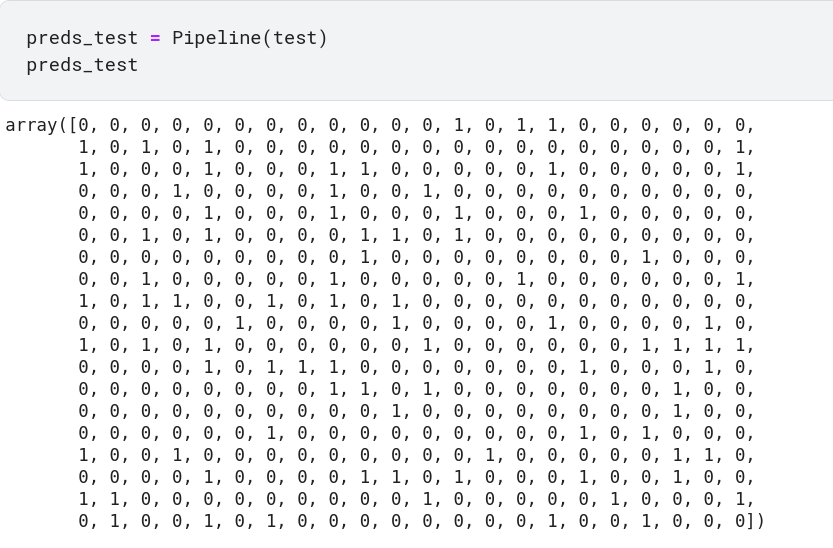
\includegraphics[width=\textwidth]{Figures/preds_teste.png}
 \caption{Predição do resultado final.}
 \label{preds_teste}
\end{figure}

\newpage
Na sequência, construímos o arquivo final \emph{submission.csv} conforme a listagem \ref{submission}. Seguindo as especificações demonstrados pelo arquivo de exemplo \emph{gender\_submission.csv} como podemos observar na Figura \ref{genderVsubmission} ambos com as mesmas colunas e passageiros. 
\begin{listing}[!ht]
\begin{minted}{Python}
pyreds_test = Pipeline(test)
#armazenamos o Array com as predições geradas pela função Pipeline

output = pd.DataFrame({'PassengerId': test.PassengerId,
                       'Survived': preds_test})
#transformamos o Array resultante em um dataframe
output.to_csv('submission.csv', index=False)
#geramos um csv a partir do dataframe
\end{minted}
\caption{Gerando o arquivo \emph{submission.csv}}
\label{submission}
\end{listing}

\begin{figure}[!h]
 \centering
 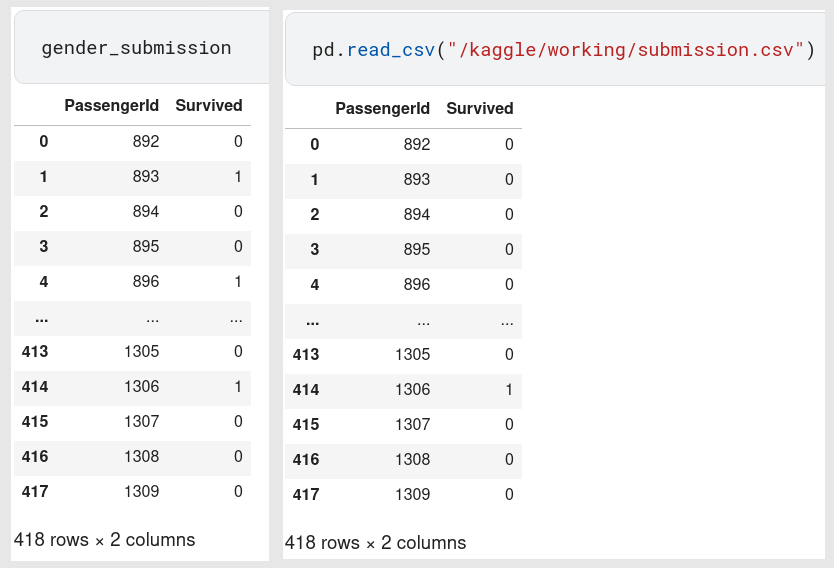
\includegraphics[width=\textwidth]{Figures/gender_output.png}
 \caption{Comparação entre nossa solução e o exemplo.}
 \label{genderVsubmission}
\end{figure}

A partir da criação do arquivo \emph{submission.csv} basta selecionarmos, na plataforma Kaggle, a opção "\emph{Competitions}" no menu à direita de nosso notebook e clicarmos na opção "\emph{submit}" apresentada na Figura \ref{submit}. A plataforma automaticamente identificará o arquivo e avaliará a solução. 
\begin{figure}[H]
\centering
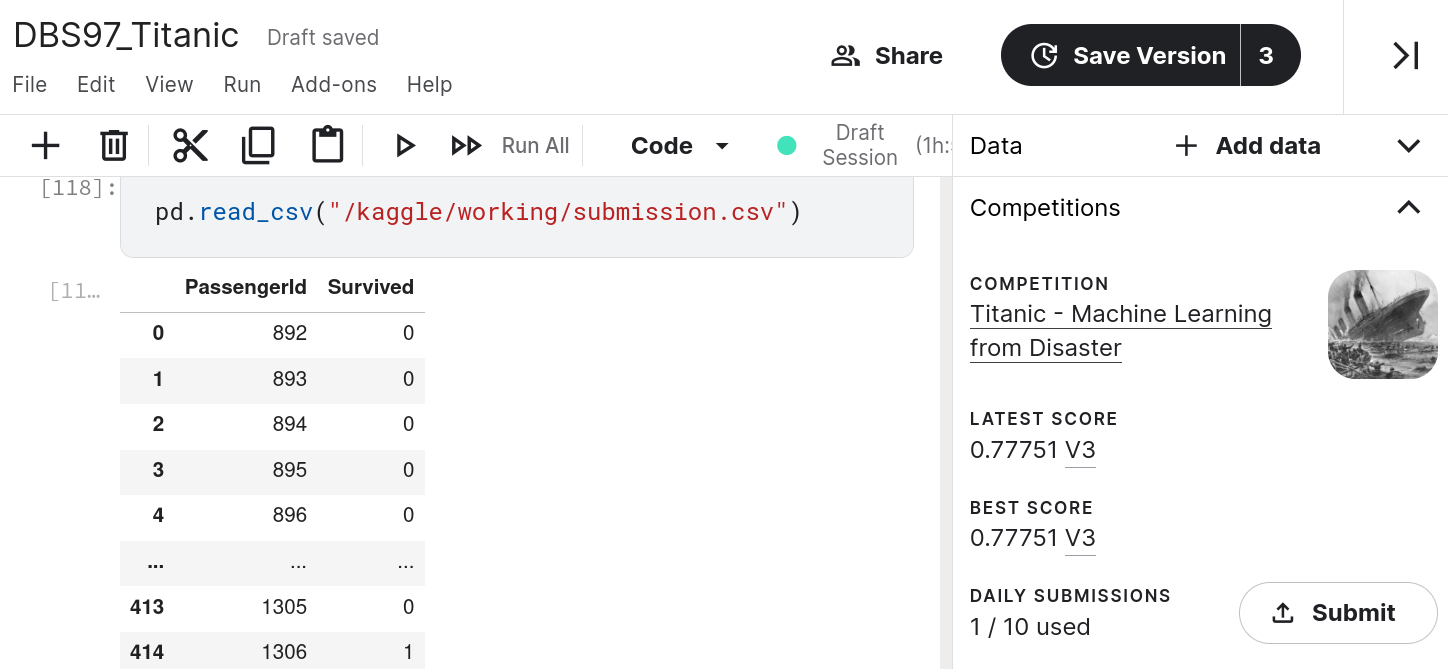
\includegraphics[width=\textwidth]{Figures/submit.png}
\caption{Submetendo o arquivo resultando ao Kaggle.}
\label{submit}
\end{figure}

\newpage
\section{Resultados}
\label{resultados}

Nesta seção apresentamos os primeiros resultados obtidos nesta pesquisa usando o Projeto Titanic da Plataforma Kaggle.

\subsection{Bases Gerais}
Nesse primeiro subprojeto buscamos estruturar uma definição para a ciência de dados a partir dos artigos estudados. 

\subsubsection{O que é Ciência de Dados?}
\cite{BATON} define a ciência de dados como o campo multidisciplinar que busca novas ideias a partir de dados do mundo real através da aplicação estruturada de técnicas primariamente estatísticas e computacionais. 
O artigo também afirma que na literatura ainda há considerável debate quanto aos contornos desse campo, porém, os especialistas tendem a concordar que a necessidade de integrar diversas disciplinas, aliada aos desafios de criar uma infraestrutura analítica robusta, introduziram um conjunto único de desafios que são melhor enfrentados por profissionais chamados "cientistas de dados". Ao que \cite{DONOHO} acrescenta:
\begin{quote}
"Ciência de Dados" é o melhor campo para acomodar pesquisa de grande impacto que seria difícil de classificar de outro modo, como por exemplo Tukey 1977 EDA e o trabalho de Wickham em Tidy Data e Grammar of Graphics.
\end{quote}

Essa nova ciência, conclamada em 1962 por John Tukey, foi recebida com timidez e controvérsia entre os estatísticos. Mas, meio século depois, com a popularização de linguagens e ambientes de programação quantitativos como o R\cite{ihaka1996r},  ela se tornou auto-evidente. Isto porque o que antes era uma descrição em prosa de uma análise, agora poderia ser precisamente descrito em um \textsc{script} com alto nível de abstração. Esses chamados \textit{workflows} podem ser compartilhados, reexecutados com outros dados, facilmente modificados e quantificados. Logo, se tornaram evidentes objetos de pesquisa, \cite{DONOHO}.

Ambos os artigos \cite{BATON,DONOHO} observaram na literatura a precisão da profecia de Tukey, especialmente em sua afirmativa sobre a Ciência de Dados ser uma disciplina orientada pela prática. Ou seja, seu sucesso deriva do valor gerado ao resolver problemas do mundo real, maximizar resultados, e a sua efetividade em gerar valor. 

\subsubsection{Processos que constituem a Ciência de dados}
Outra dimensão ressaltada por Tukey e observada por \cite{DONOHO} especialmente nas ideias de John Chambers\cite{CHAMBERS} and Bill Cleveland\cite{cleveland2001data} é a ciência que se forma no entorno do "aprender com dados do mundo real" e tudo que esse processo engloba. Especialmente a possibilidade da Ciência de Dados construir e oferecer ferramental que possibilite o avanço de todas as outras ciências, ao aprimorar todo o processo de transformar dados em informação, desde ferramentas de processamento computacional, até bases epistemológicas desse processo. 

\cite{DONOHO} chama essa disciplina expandida de \textit{Greater Data Science (GDS)}, e a divide em seis sub-áreas:
\begin{enumerate}
\item Data Gathering, Preparation, and Exploration
\item Data Representation and Transformation
\item Computing with Data
\item Data Modeling 
\item Data Visualization and Presentation
\item Science about Data Science

\end{enumerate}
Já \cite{BATON} traz uma abordagem observacional, processando o que já está registrado na literatura com pesquisas de mercado. O artigo sintetiza o Modelo de Trabalho ou \emph{Data Work Model}, constituído de quatro processos de alta ordem, divididos em 14 subprocessos da seguinte forma:
\begin{itemize}
\item \textbf{Preparation}: Defining Needs, Data Gathering, Data Creation, Profiling, and Data Wrangling
\item \textbf{Analysis}: Experimentation, Exploration, Modeling, Verification, and Interpretation.
\item \textbf{Deployment}: Monitoring and Refinement
\item \textbf{Communication}: Dissemination and Documentation
\end{itemize}

O artigo também identifica mais dois processos de alta ordem emergindo:
\begin{itemize}
\item \textbf{Pedagogy} 
\item \textbf{Collaboration}
\end{itemize}

Podemos observar que ambas as definições são compatíveis e adequadas à sua proposta: a GDS \cite{DONOHO} como orientação teórica de pesquisa e organização da literatura, enquanto o Data Work Model \cite{BATON} oferece uma excelente estrutura para abordar um projeto de dados. 

\subsection{Definição de problemas de dados}
\subsubsection{Principais conceitos}\label{principais.conceitos}
 O livro \cite{DATAPYTHON} ressalta a importância fundamental de se entender o "problema do negócio" e circunscreve-lo em uma definição matemática. O que muitas vezes significa ter um papel fundamental na definição do "que será feito e como será feito". Portanto, a ciência de dados requer um diálogo imprescindível entre o cientista e pessoas especializadas na área do "negócio".
 
Nesse sentido, segundo o modelo \cite{BATON}, a definição do problema de dados é o processo de traduzir objetivos analíticos, geralmente definidos pelas parte interessadas, em um conjunto de requerimentos viáveis. Dentre tais requerimentos estão:
\begin{itemize}
\item Dados necessários
\item Planos para analisá-los
\item Definir quais serão as entregas, como por exemplo: relatórios, modelos e infraestrutura computacional. 
\end{itemize}

\subsubsection{Titanic}

No projeto Titanic, e nas competições Kaggle em geral, já temos o "problema de negócio" definido. Nesse caso, nosso problema é determinar a partir dos seus dados, quais passageiros sobreviveriam ao trágico acidente, tendo em vista, especialmente um olhar crítico para os resultados, analisando quais foram as características dos passageiros que aumentaram suas chances de sobrevivência.

A partir desse problema devemos pensar em quais dados precisamos obter para aborda-lo. Nesse caso, precisamos de uma amostra com os dados de diversos passageiros e o seu destino. Podemos utilizar tal amostra para treinar um modelo preditivo que possa receber outro conjunto análogo apenas com as informações e predizer o destino de cada um. Dessa forma, no processo de construção desse modelo esperamos compreender quais foram os fatores que mais contribuíram para o desfecho de cada pessoa à bordo. 

Já temos nessa etapa da definição do problema, conceitos iniciais de \textit{Aprendizado de Máquina}. Isto porque temos uma variável a ser predita, também chamada de variável alvo (\textbf{target}), variável resposta ou \textbf{y}. 
Para predize-la, temos um conjunto de \textbf{features}, isto é, as características de cada passageiro em nosso conjunto de dados, também chamado de \textit{DataFrame ou DataSet}. A partir das \emph{features}, geramos um conjunto de variáveis \textbf{X} para prever nossa variável \textbf{y}. 
Dessa forma, precisamos de um \emph{dataset} com \emph{features} e variável alvo. 
Estes dados de treino são inseridos em um modelo que tentará modelar matematicamente as relações de X para y, de modo que posteriormente para qualquer outro conjunto análogo a X, o modelo possa prever um valor de y. 

Assim, sabemos que devemos construir um modelo preditivo de classificação, que para cada conjunto de dados $X_i$ de um passageiro \emph{i}, ele possa gerar um $y_i$ de valor zero ou um, representando a sua sobrevivência. Também sabemos que se faz necessário, portanto, obtermos um \emph{dataset} com X e y para treinarmos nosso modelo. O que também já nos aponta para o uso da biblioteca Pandas para estruturar esse X além do uso da biblioteca \emph{Scikit Learn} para criar, treinar e utilizar um modelo de Aprendizado de Máquina em português.

\subsection{Obtenção de Dados}
\subsubsection{Conceitos principais}
Uma vez definidos os requerimentos, o passo seguinte de acordo com o modelo \cite{BATON}, é a obtenção de dados. Para tanto, o modelo ressalta três possibilidades:
\begin{itemize}
\item Identificar o conjunto de dados adequado dentre vários candidatos. 
\item Gerar novos dados a partir da integração e transformação de dois ou mais conjuntos existentes. 
\item Desenvolver critérios e mecanismos para coletar dados que ainda não existem. 
\end{itemize}
 
Tanto a primeira, quanto a segunda situação se referem aos casos nos quais o "cliente" do serviço de dados já dispõem de um banco de dados estruturado. Nesse caso, normalmente, a obtenção envolve escrever uma \emph{query} na linguagem SQL.  
 Do contrário, quando o cliente dispõem dos dados porém em formato inadequado,  é necessário primariamente adequá-los ao primeiro caso, o que normalmente também envolverá a linguagem SQL, provavelmente \emph{scritps} e possivelmente certa organização manual de dados.  

 No terceiro caso, há uma variedade maior de possibilidades, desde a realização de pesquisa como questionários, até a criação de \emph{scritps} para capturar da internet as informações relevantes, processo que chamamos de \emph{Webscrapping}\cite{mitchell2018web}. 
  
O livro \cite{DATAPYTHON} também ressalta a importância da documentação do conjunto de dados obtidos. Nela devem estar as principais informações sobre o \emph{dataset}, tais como a explicação de suas colunas e seus conteúdos, definições de termos, seu contexto, dentre outras. 

 \subsubsection{SQL}
Conforme mencionamos na metodologia, a linguagem SQL não foi necessária no projeto Titanic, entretanto muitos autores como \cite{SCRATCH,DATAPYTHON} ressaltam a sua importância, especialmente no ferramental de um cientista de dados. \cite{debarros2022practical} a define da seguinte maneira:
\begin{quote}
    SQL é uma linguagem de programação amplamente utilizada que permite definir e consultar bancos de dados. Seja você um analista de marketing, um jornalista ou um pesquisador mapeando neurônios no cérebro de uma mosca, você se beneficiará do uso do SQL para gerenciar objetos de banco de dados, bem como criar, modificar, explorar e resumir dados. 
\end{quote}

Nesse sentido, elencamos recursos para aprender essa habilidade que esperamos nos aprofundar nos próximos trabalhos. Identificamos os livros \cite{debarros2022practical,Silberschatz2019DBS} como as referências interessantes. Além deles, acreditamos que a forma mais eficiente de se aprender uma habilidade prática é por meio da prática direcionada, nesse sentido, os seguintes sites se mostraram os mais eficientes em apresentar exercícios práticos: 
\begin{itemize}
\item \href{https://sqlbolt.com/}{SQLbolt} \footnote{sqlbolt.com/}
\item \href{https://www.hackerrank.com/domains/sql}{Hacker Rank}\footnote{www.hackerrank.com/domains/sql}
\item \href{https://pgexercises.com/}{PostgreSQL Exercises}\footnote{pgexercises.com}
\end{itemize}
 
 \subsubsection{Titanic}
À partir da definição do problema, buscamos obter os dados disponíveis ou criá-los. No caso de nosso projeto Titanic, como em todas as competições Kaggle, os dados são disponibilizados pela plataforma e podem ser obtidos conforme descrito na metodologia. Temos, portanto, os \emph{DataFrames}  para o treinamento e validação do modelo, predição e submissão à plataforma Kaggle e exemplo de submissão derivados dos arquivos \emph{train.csv, test.csv, e gender\_submission.csv} respectivamente apresentados nas Figuras \ref{df.csv}, \ref{test.csv} e \ref{gender.submission.csv} respectivas. 
\begin{figure}[H]
\centering
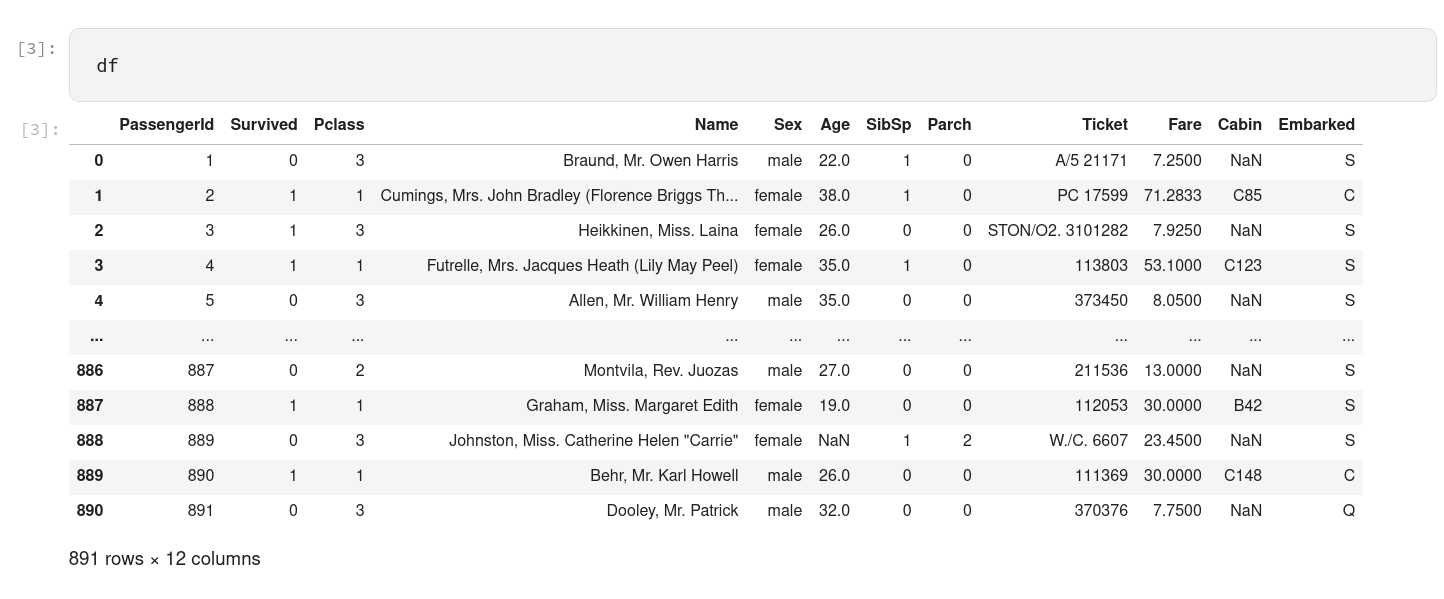
\includegraphics[width=\textwidth]{Figures/df.png}
\caption{\emph{DataFrame} treinamento lido do arquivo train.csv}
\label{df.csv}
\end{figure}
\begin{figure}[H]
\centering
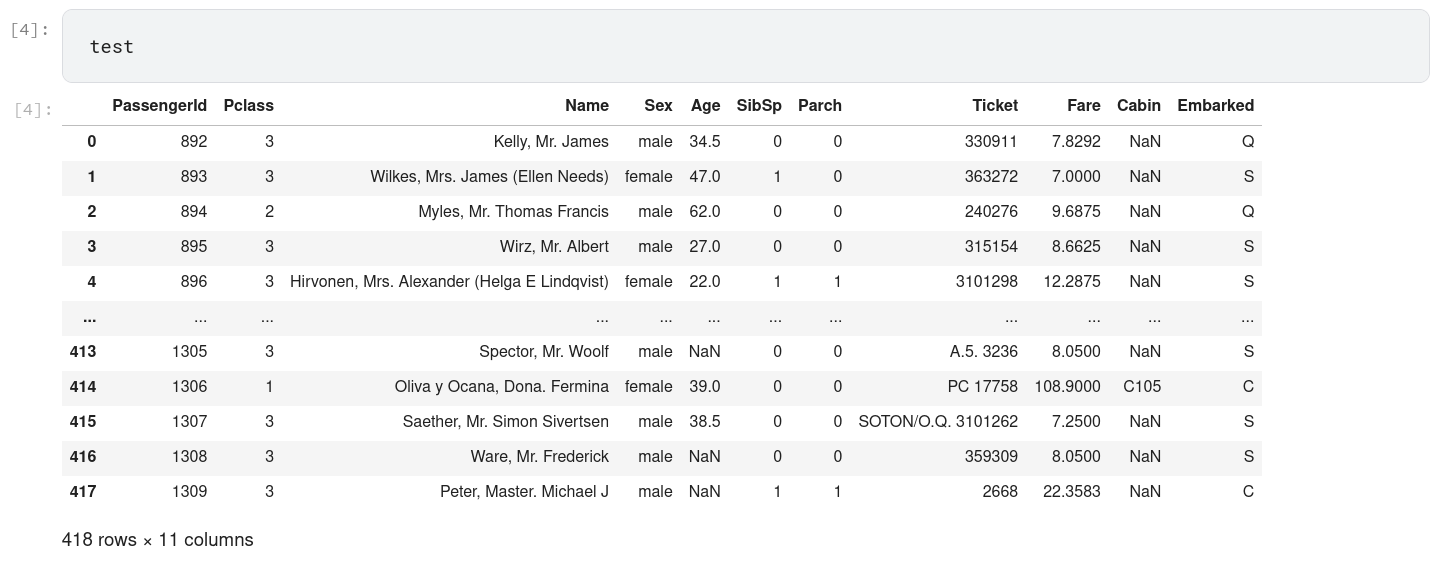
\includegraphics[width=\textwidth]{Figures/test.png}
\caption{\emph{DataFrame} do arquivo test.csv, que será predito e submetido à plataforma}
\label{test.csv}
\end{figure}
\begin{figure}[H]
\centering
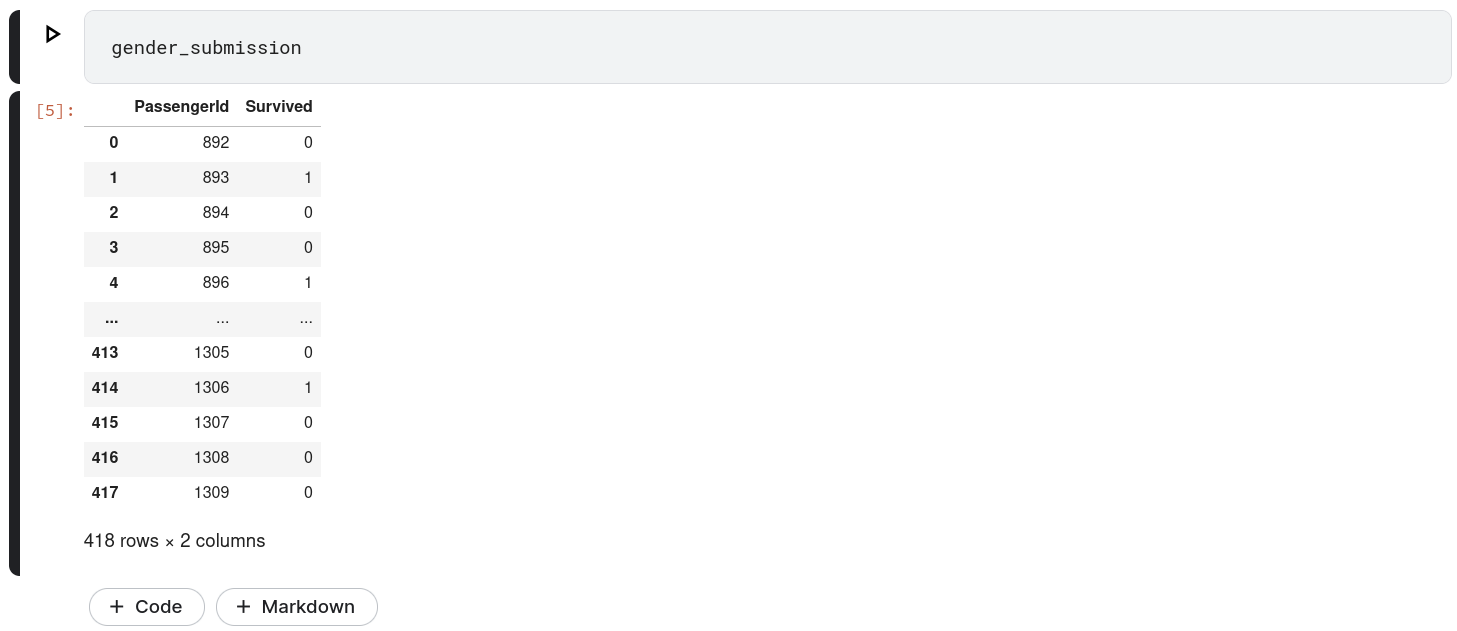
\includegraphics[width=\textwidth]{Figures/gender_submission.png}
\caption{\emph{DataFrame} gender\_submission.csv submetido à plataforma Kaggle}
\label{gender.submission.csv}
\end{figure}

\begin{itemize}
\item \emph{train.csv}:  uma tabela com 891 linhas e 12 colunas, respectivamente representando cada passageiro, e suas \emph{features}, inclusive se ele sobreviveu. Exatamente o \emph{dataset} descrito em nosso requerimento, portanto será o nosso principal \emph{DataFrame} de trabalho, que iremos analisar, transformar e utilizar para treinar nosso modelo preditivo.  
\item \emph{test.csv}: muito semelhante ao arquivo anterior, contem outros 418 passageiros, mas dessa vez apenas 11 colunas. Isto porque a coluna "\textsc{survived}" está ausente, exatamente a coluna que nosso modelo se propõe a preencher. Este, é o conjunto de dados cuja resposta será utilizada na avaliação automática que o kaggle faz em nosso modelo. 
\item \emph{gender\_submission.csv}: é um exemplo de submissão a competição kaggle, ela contém as mesmas 418 linhas e a mesma coluna "\textsc{PassengerId}" que o arquivo \emph{test.csv} contém, acrescida da coluna "\textsc{Survived}", nesse caso, preenchida a título de exemplo de modo que todas as passageiras sobreviveram e todos os passageiros morreram. Esse é um exemplo do arquivo que será submetido a competição e utilizado para avaliar nossa solução para o problema. 
\end{itemize}

\subsection{Data Analysis}
\subsubsection{Conceitos principais}
\cite{BATON} aponta que esse processo, denominado de Data Analysis pelo livro \cite{DATAPYTHON}, também pode ser encontrado com outros nomes na literatura como "pré-processamento", "tidying", "limpeza", "wrangling", "Exploratory Data Analysis (EDA)" ou ainda "Data Understanding". 
Nesse sentido, as autoras defendem dividi-lo entre "Profiling" e "Data Wrangling" e agrupa-los junto aos passos anteriores, de modo a constituir o macro processo de "Preparation". 

Assim, de acordo com o modelo apresentado, temos as seguintes definições:
\begin{itemize}
\item \textbf{Profiling}: é o processo de avaliar atributos dos dados para entender a distribuição de seus valores, identificar valores faltantes e examinar a sua associação à outros atributos. Bem como compreender os dados e seu conteúdo. 
\item \textbf{Data Wrangling}: processo de utilizar o que foi aprendido no Profiling para conformar e transformar os dados de modo a adequá-los para os próximos passos. 
\end{itemize}

Nesse sentido, dentro do ecossistema Python, a biblioteca Pandas é a ferramenta absoluta para manipulação de tabelas, aliada a NumPy, que traz um robusto repertório de implementações matemáticas e aplicações de álgebra linear.\cite{PRINCIPLES}

\subsubsection{Técnicas}
Segundo \cite{BATON,DONOHO,DATAPYTHON} Essa etapa é sabidamente a mais dispendiosa de um projeto de dados. Devido principalmente ao tempo necessário e dificuldade de automatizar. Dessa forma, é também uma das etapas mais difíceis de se ensinar justamente em função da intervenção humana e seu processo quase artesanal para compreender adequar os dados. 

Dessa forma, segundo \cite{DATAPYTHON}, devemos analisar os dados tanto diretamente quanto por meio de sumários gráficos e numéricos, mas principalmente analisar criticamente se nossos achados fazem sentido, e se estão de acordo com a documentação do dataset. Nesse sentido compilamos a seguinte lista de perguntas para nortear o processo de \emph{Profiling}:
\begin{enumerate}
\item Quantas colunas? (podem ser features, variável resposta, ou metadados)
\item Quantas linhas? (checar se cada linha é uma amostra)
\item Quais são os tipos de features? Quais são categóricas e quais são numéricas? 
\item Como são esses dados? (em numéricas podemos examinar range de valores, ou frequência de diferentes classes em categóricas por exemplo)
\item Temos valores faltantes? 
\end{enumerate}
Se o dataset for pequeno o bastante podemos examinar individualmente cada feature. Já quando o dataset tem centenas de features devemos explorar técnicas de redução de dimensionalidade, que condensam informação em um número menor de features derivadas ou métodos de feature selection que podem auxiliar a encontrar features importantes dentre muitas candidatas. Nesse sentido, \cite{DATAPYTHON} afirma:
\begin{quote}
    "Tempo dedicado analisando critica e detalhadamente se um dataset cumpre seu propósito é um tempo bem gasto." 
\end{quote}

\subsubsection{Titanic}
No projeto Titanic, portanto, iniciamos o \emph{Profilling} do nosso arquivo principal \emph{train.csv}, por meio da variável "\textsc{df}" orientados pela lista de perguntas que construímos.

Como podemos observar na Figura \ref{df.info}, temos 12 colunas ou \emph{features} e 891 linhas ou \emph{dados}. Também logo observamos que as colunas \textsc{Age, Cabin} e \textsc{Embarked} tem dados faltantes. As outras 9 \emph{features} estão totalmente preenchidas. 
Observamos por meio do atributo \emph{Dtype} que as colunas \textsc{Name, Sex, Ticket, Cabin} e \textsc{Embarked} são variáveis categóricas (definidas como tipo \emph{object}), enquanto as outras são numéricas. Podemos confirmar tal fato observando os conteúdos da tabela de treinamento mostrada na Figura \ref{df.csv} onde podemos ver as primeiras e últimas entradas desta tabela de treinamento.
\begin{figure}[H]
\centering
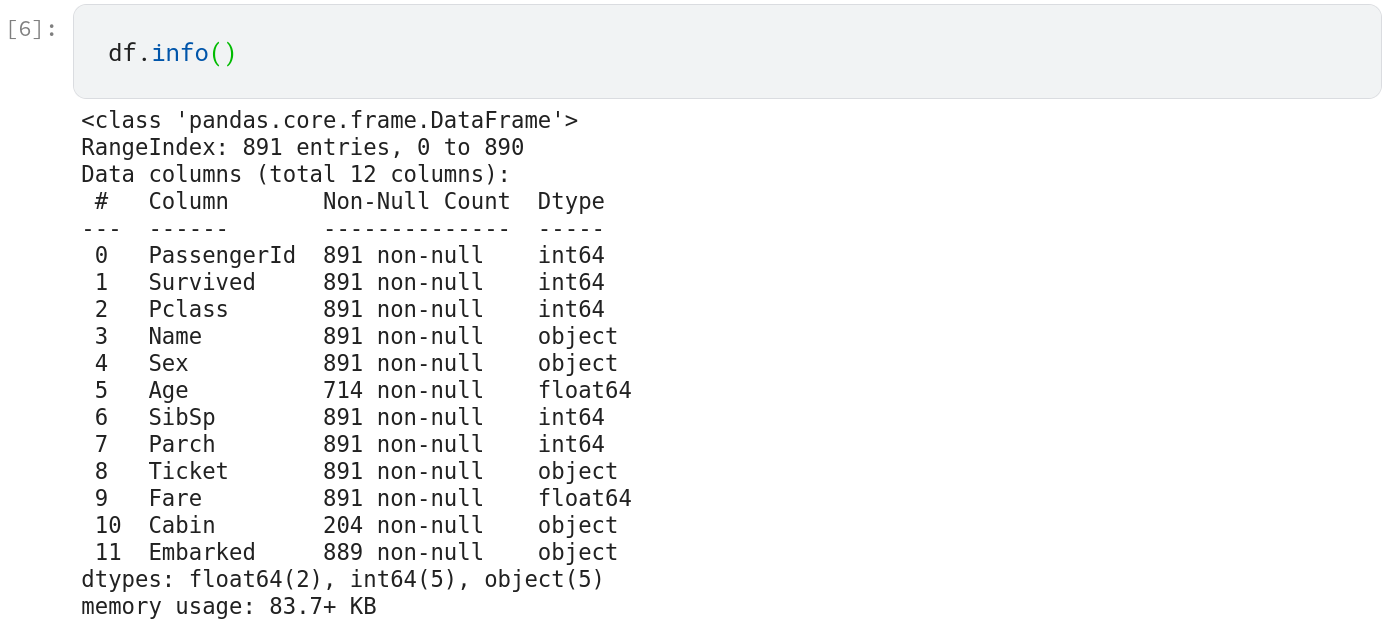
\includegraphics[width=\textwidth]{Figures/df.info().png}
\caption{\label{df.info}Informação sobre a tabela de treinamento, usando o comando \textsc{df.info()}}
\end{figure}

Logo em seguida observamos a tabela \textsc{df} e estudamos a documentação do \emph{DataSet} para compreender cada uma das 12 colunas/features. Na sequência apresenta-se o significado de cada uma destas colunas no Projeto Titanic:
\begin{itemize}
\item \textsc{PassengerId}: o número que representa cada passageiro. 
\item \textsc{Survived}: 0 ou 1, para representar se determinado passageiro sobreviveu.
\item \textsc{Pclass}: classe do ticket do passageiro. Equivalente a classe economica 1-alta;2-media;3-baixa
\item \textsc{Name}: nome do passageiro com sobrenome e pronome de tratamento. 
\item \textsc{Sex}: masculino ou feminino. 
\item \textsc{Age}: idade em anos, em bebês abaixo de 1 ano é uma fração estimada. 
\item \textsc{SibSp}: \# irmãos e cônjuges a bordo.
\item \textsc{Parch}: \# paretens e filhos a bordo. 
\item \textsc{Ticket}: número do ticket
\item \textsc{Fare}: Tarifa paga pelo passageiro. 
\item \textsc{Cabin}: Número da cabine. 
\item \textsc{Embarked}: Porto de embarque. C = Cherbourg, Q = Queenstown, S = Southampton
\end{itemize}

Na sequência, analisamos suas principais métricas (média, desvio padrão, quartis). Na Figura \ref{df.describe} se apresenta o resultado da execução do comando \textsc{df.describe()}.
\begin{figure}[H]
\centering
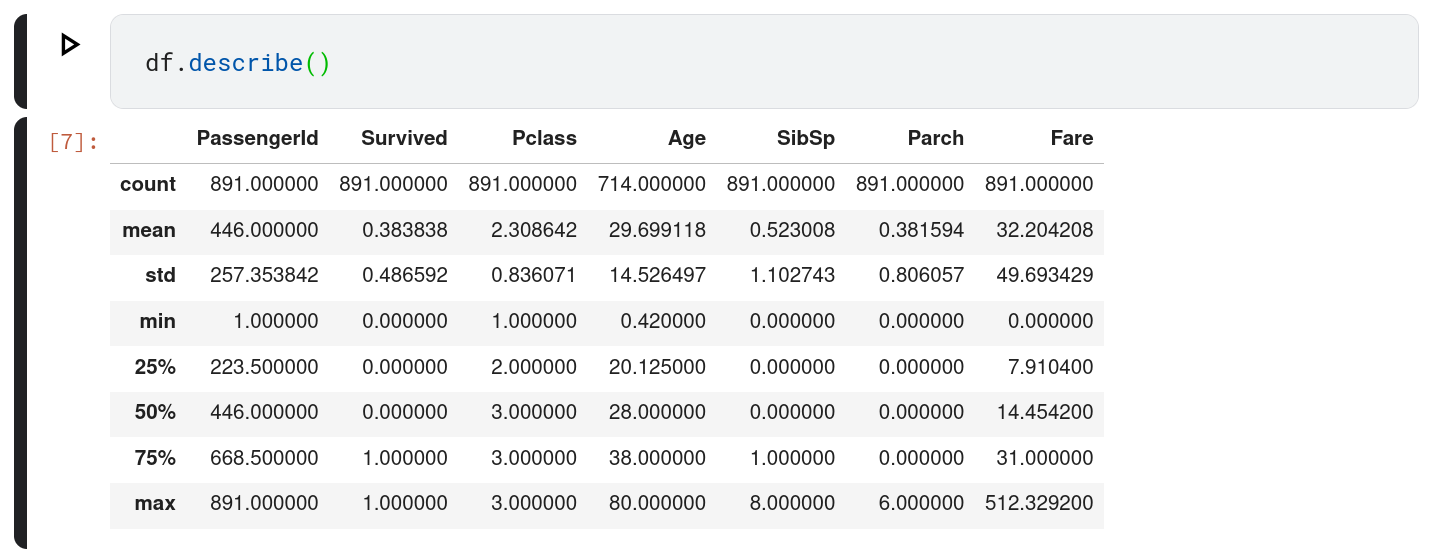
\includegraphics[width=\textwidth]{Figures/df.describe().png}
\caption{\label{df.describe}Estatística descritiva dos dados do treinamento.}
\end{figure}

A partir dessas observações podemos desenvolver as seguintes suposições:
\begin{itemize}
\item \textsc{PassengerID} pode ser desconsiderada, uma vez que é apenas um artefato computacional para denominar as colunas.
\item \textsc{Name} a princípio também será desconsiderado, uma vez que é pouco provável que tenha uma relação direta com a sobrevivência portanto a complexidade de quantificá-la não parece valer. 
\item \textsc{Sex} pode ser convertida em 0 e 1. 
\item \textsc{Age} tem um número considerável de linhas com dados faltantes, poderíamos excluí-la, porem faria sentido a idade ter alguma relação com a sobrevivência, nesse caso iremos lidar com os valores faltantes. Também podemos criar uma \emph{Feature} com intervalos de idade. 
\item \textsc{SibSp} e \textsc{Parch} podem ser combinados em uma terceira \emph{feature} que combina os familiares à bordo, seria interessante saber se deveríamos somar ou multiplicar esses números. 
\item \textsc{Ticket} também pode ser, a princípio, desconsiderado, uma vez que não temos na documentação a explicação de seu código alfa numérico, e assim como \textsc{Name}, essa \emph{feature} não parece ter direta relação com a sobrevivência. 
\item  \textsc{Fare}, parece bem promissora, uma vez que não apresenta dados faltantes, já é numérica, e parece ter uma relação clara com a sobrevivência.  
\item \textsc{Cabin}, assim como \textsc{ticket}, não temos uma tradução numérica, poderíamos construir uma \emph{Feature} como a contagem de cabines, entretanto temos muitos valores faltantes, portanto, é provável que desconsidera-la seja a melhor opção. 
\item \textsc{Embarked}, pode ter alguma relação coma sobrevivência, provavelmente a trataremos. 
\end{itemize}

Podemos utilizar a pivotagem pra nos indicar a importância relativa de nossas \emph{features} numéricas, ou seja, agrupar cada uma delas de acordo com a sobrevivência por meio de suas médias. Assim teremos para cada coluna o seu valor médio entre os sobreviventes e entre os não sobreviventes, desse modo, variáveis que foram importantes como mostram as Figuras \ref{df.groupby} e \ref{embarked.groupby}.

\begin{figure}[H]
\centering
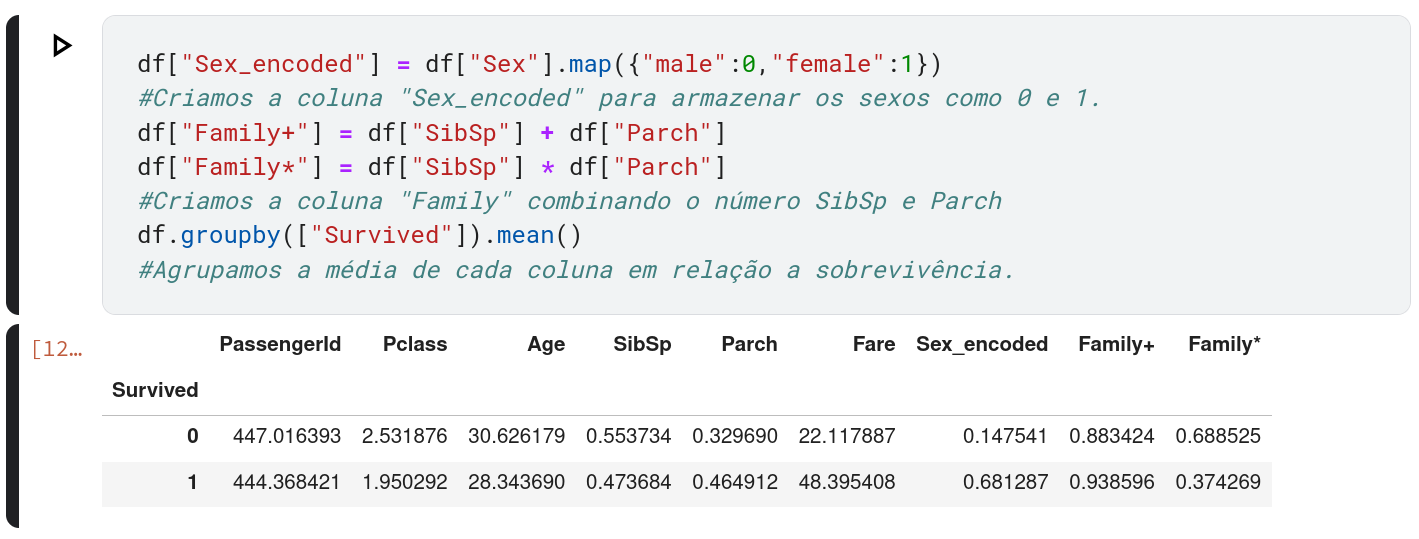
\includegraphics[width=\textwidth]{Figures/df.groupby.png}
\caption{\label{df.groupby}Agrupando cada coluna em média de acordo com a sobrevivência.}
\end{figure}

\begin{figure}[H]
\centering
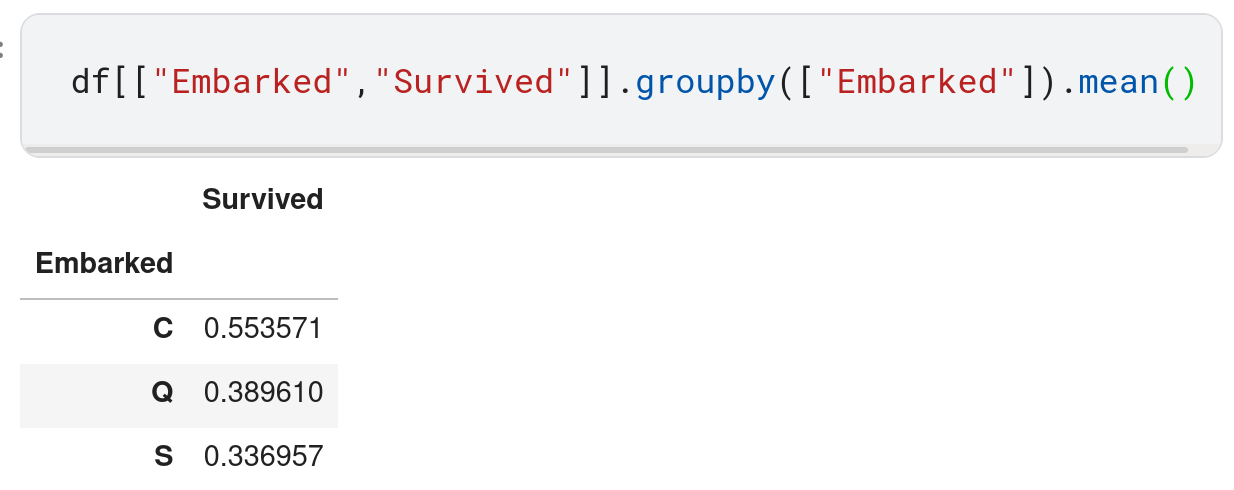
\includegraphics[width=\textwidth]{Figures/embarked.png}
\caption{\label{embarked.groupby}Agrupando a sobrevivência de acordo com os portos de embarque.}
\end{figure}

A partir dela podemos constatar que a média de classe, sexo e custo da passagem foi bem diferente entre os que sobreviveram e os que não sobreviveram, o que sugere serem variáveis importantes. O número de irmãos e cônjuges, bem como o número de pais e filhos apresentaram uma diferença mais sutil, assim como a idade. Pode ser entretanto que haja alguma relação de grupos dessas \emph{features} com a sobrevivência, conforme observamos na Figura \ref{age.hist} ao compararmos os histogramas das idades dos sobreviventes com o histograma das idades das vitimas. 
Também podemos observar nas Figuras \ref{family.groupby} e \ref{df.groupby.plot} a existência de algum padrão de sobrevivência de acordo com a quantidade de parentes a bordo. 
\begin{figure}[H]
\centering
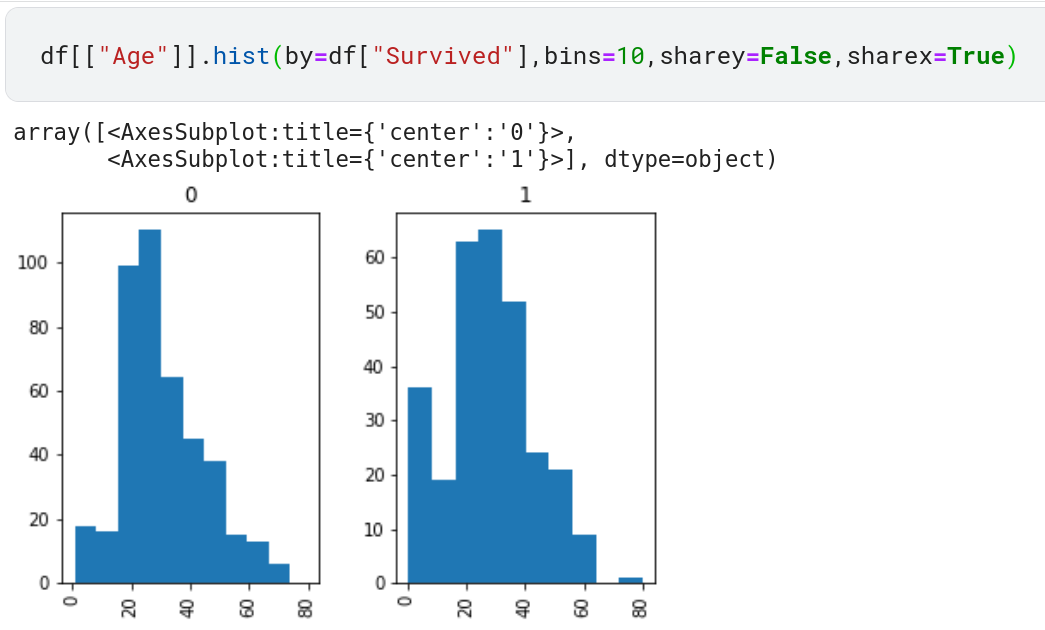
\includegraphics[width=\textwidth]{Figures/age.hist.png}
\caption{Histograma das idades dos sobreviventes e das vítimas.}
\label{age.hist}
\end{figure}

\begin{figure}[H]
\centering
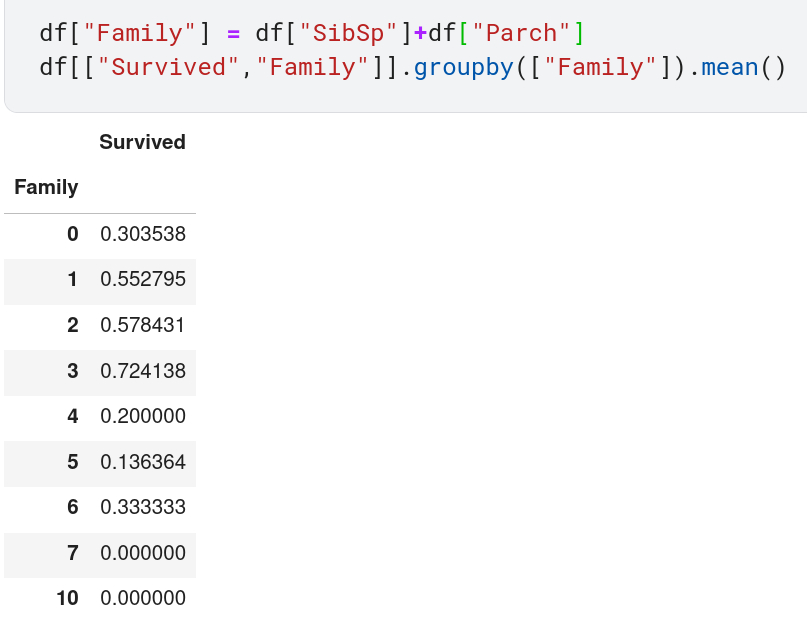
\includegraphics[width=\textwidth]{Figures/family_groupby.png}
\caption{\label{family.groupby}Índice de sobrevivência para cada quantidade de parentes a bordo.}
\end{figure}
\begin{figure}[H]
\centering
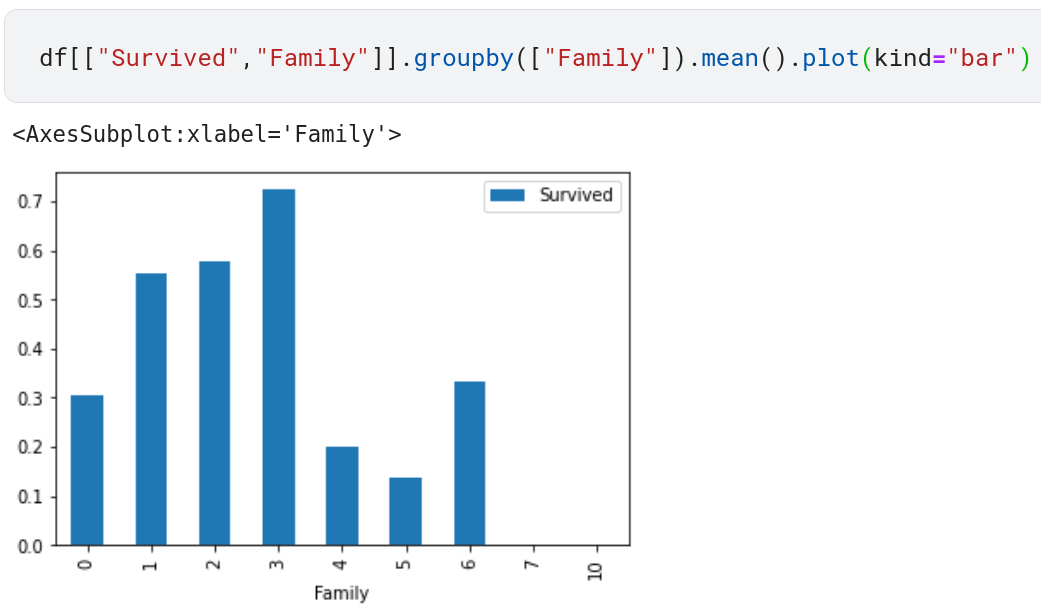
\includegraphics[width=\textwidth]{Figures/family_survivor_plot.png}
\caption{\label{df.groupby.plot}Gráfico do índice de sobrevivência para cada quantidade de parentes a bordo.}
\end{figure}

Assim, concluímos o seguinte:
\begin{itemize}
\item Removeremos as colunas: \textit{PassengerId, Name, Ticket} e \textit{Cabin}. 
\item Pclass já pode ser utilizada conforme se encontra.
\item Modificaremos a feature Sex codificando os valores male e female para 0 e 1 respectivamente. 
\item Completaremos os valores faltantes da Age considerando a mediana da o sexo e a classe do passageiro do passageiro. 
\item Criaremos a feature Family combinando Parch e SibSp e a codificaremos numericamente. 
\item Fare, assim como Pclass já está pronta para ser utilizada. 
\item Codificaremos os portos em Embarked.
\end{itemize}

Finalmente, uma vez que estabelecemos um plano, podemos aplicá-lo ao nosso dataframe \textsc{df}. Um ponto muito importante é que devemos estruturar as transformações de modo que possam ser aplicadas tanto nos dados de treino quanto nos dados que o modelo receberá em produção. Desse modo, obtemos nosso dataset tratado, conforme temos na Figura \ref{wranglin.results}.

\begin{figure}[H]
\centering
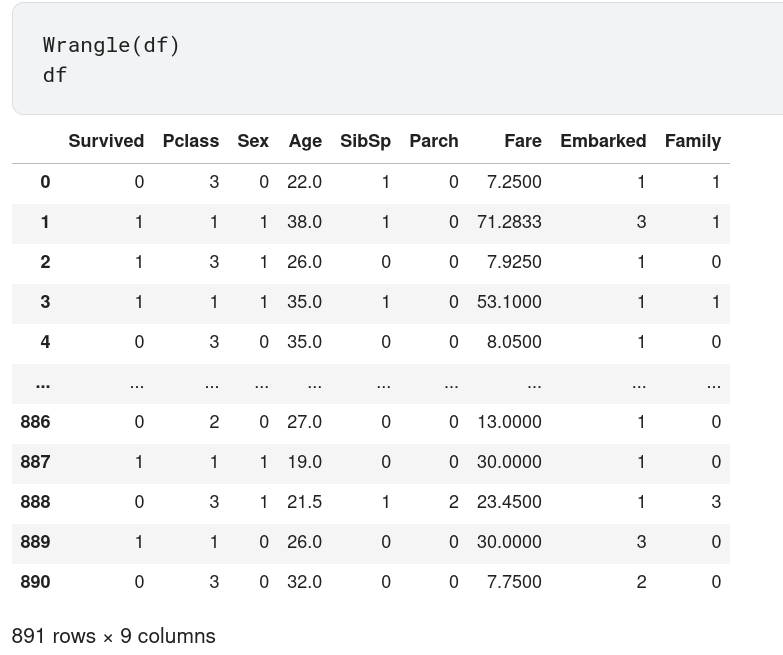
\includegraphics[width=\textwidth]{Figures/wrangle_results.png}
\caption{\label{wranglin.results}Aplicação da função \emph{Wrangle()} para preprocessar os dados de treinamento.}
\end{figure}

\subsection{Aprendizado de Máquina}
\subsubsection{Conceitos Principais}
No modelo \cite{BATON}, após o macroprocesso de \textit{Preparation} temos o macroprocesso \textit{Analysis}. Dessa forma, essa etapa que chamamos de \textit{Aprendizado de Máquina} é equivalente aos seguintes processos da pipeline:
\begin{itemize}
\item \textbf{Modeling}: aplicar técnicas computacionais e estatísticas para derivar informação que oriente possíveis ações a partir dos dados. 
\item \textbf{Verification}: é o processo avaliativo para confirmar a robustez dos resultados do código e dos modelos. É interessante notar que tem crescido a importância também de considerar a transparência e imparcialidade (fairness) dos processos de dados. 
\item \textbf{Interpretation}: processo de compreensão dos resultados, da exploração e do modelo no que diz respeito as suas aplicações no mundo real.
\end{itemize}

As principais ferramentas desse etapa no ecossistema Python são:
\begin{itemize}
\item Bibliotecas Pandas e NumPy utilizadas, assim como na etapa anterior, para manipulação de tabelas e operações com colunas.
\item \textit{Scikit Learn}: é a principal biblioteca para aprendizado de máquina em Python. Podemos utiliza-la para facilmente criar modelos dentro dos diversos tipos oferecidos. Ela também oferece ferramentas para suportar todo o processo de treiná-los, avalia-los, ajustá-los e utilizá-los. Além ser open source e de oferecer diversas outras funcionalidades como a criação de pipelines de processamento automatizado. [citar a própria página oficial do projeto] 
\end{itemize}

Nesse contexto, quando falamos de \textit{Aprendizado de Máquina} (ML), nos referimos a modelos preditivos que "aprendem" a partir de dados. Normalmente, os modelos encontram as relações e correlações entre colunas de uma tabela. Nesse sentido, podemos definir um modelo como a especificação de uma relação matemática ou probabilística entre variáveis,  \cite{SCRATCH} \cite{PRINCIPLES}.

\cite{PRINCIPLES} Ressalta as seguintes premissas universais a todos os modelos de ML:
\begin{itemize}
\item Os dados de entrada devem ser limpos e pré processados. Poucos modelos toleram dados sujos, com valores faltantes ou variáveis categóricas. Nesse sentido, parte importante da preparação dos dados envolve lidar com essas questões.
\item Em geral, são muito sensíveis a dados ruidosos. 
\item Cada linha da tabela representa uma única observação do ambiente que tentamos modelar. 
\item  Deve existir alguma relação entre variáveis.
\item Modelos são geralmente considerados semi-automáticos, isto é, necessitam que humanos tomem decisões. Seu output é normalmente uma sequência de números. Um ser humano é necessário para analisar esses resultados com a perspectivas adequadas e comunica-los.
\end{itemize}

Nesse sentido, \cite{SCRATCH} elenca os seguintes conceitos fundamentais à modelagem de dados:
\begin{itemize}
\item Overfitting e Underfitting: é a medida do quanto o modelo é capaz de aprender e generalizar determinado conjunto de dados. Overfitting ocorre quando o modelo "decora" os dados de treino, portanto ele tem um excelente rendimento com dados conhecidos e péssimo com dados novos. Underfitting quando ele não aprende o suficiente.
\item Bias-Variance trade off: analoga ao over e underfitting, um modelo com Bias alta performa mal até mesmo nos dados de treino (underfitting), enquanto uma variança alta significa que dados diferentes levariam a modelos muito diferentes, o que corresponde ao overfitting.
\item Correctness: Existem diversas métricas para se avaliar um modelo. Normalmente se utiliza Acurácia,  Precision and Recall, muitas vezes a sua média harmônica denominada F1-score. 
\item Feature selection, extraction e engineering: um dos conceitos mais importantes de um modelo são as suas features, a seguir detalhamos seus principais conceitos e técnicas.
\end{itemize}

\subsubsection{Feature Engineering} \label{feature-Eng}
O objetivo do Feature Engineering é aumentar a performance preditiva do modelo, diminuir a necessidade computacional e de dados, e finalmente melhorar a interpretabilidade dos resultados. Nessa sessão abordamos os principais fundamentos, e a práticas na preparação das features de um modelo. 

Nesse sentido, \cite{SCRATCH} ressalta os seguintes pontos centrais:
\begin{itemize}
\item Features são quaisquer inputs do nosso modelo. 
\item Quando nossos dados têm poucas features o modelo tende ao underfit. Do mesmo modo que o excesso de features faz com o que o modelo overfite. 
\item Existem três tipos principais: booleano (0 ou 1), numérico e categórico (uma escolha dentro um conjunto discreto de opções).
\item O tipo das features pode restringir o tipo de modelo que pode ser usado. Como por exemplo os modelos de regressão requererem dados numéricos, enquanto árvores de decisão conseguem lidar tanto com dados numéricos quanto categóricos.
\end{itemize}

Dentre as práticas mais importantes nesse processo de construção das features de um modelo podemos citar:
\begin{itemize}
\item Compreender as features, estudar o dataset e sua documentação, pesquisar o problema a ser solucionado tanto com profissionais da área quanto por meio de livros e artigos. Relações numéricas entre features são normalmente expressas por fórmulas matemáticas. Frequentemente as descobrimos quando pesquisamos a área do problema.
\item Estudar outras soluções para problemas similares, ou anteriores.
\item Usar a visualização de dados. A visualização muitas vezes pode revelar patologias em uma distribuição, ou inspirar possíveis simplificações para relações complicadas, ou ainda sugerir algum tipo de transformação como por exemplo aplicar uma função logarítmica. 
\item Podemos utilizar uma função para medir a relação de determinada feature com a variável alvo e desse modo rankea-las para facilitar a busca das  features mais interessantes. Mutual Information é um exemplo de métrica utilizada nesse sentido, semelhante a correlação estatística, ela tem a vantagem de conseguir medir qualquer relação, não apenas linear entre variáveis. 
\item A utilidade de uma feature, entretanto, é diretamente proporcional a capacidade do modelo aprender a relação dela com a variável alvo. Desse modo, mesmo features com alto índice de relação com a variável alvo, podem precisar serem transformadas para expor ao modelo a sua associação a variável alvo. Quanto mais complexa a combinação, mais difícil para o modelo aprender a relação.
\end{itemize}

Além das práticas podemos citar as seguintes principais técnicas para abordar esse processo:
\begin{itemize}
\item Aplicação de uma potência, raiz, ou transformar valores absolutos em percentual ou proporções
\item Normalização. Isto é, deslocar a distribuição dos dados de modo que sua média seja zero e escalar seus valores de modo que seu desvio padrão seja unitário. 
\item Criação de uma feature de contagem. Podemos agregar o número de fatores de risco, o número de ingredientes, etc.
\item Frequentemente temos features complexas que podem ser separadas em features menores, como números de telefone (operadora e número), endereço (rua, cidade, país). Da forma semelhante podemos ter features que poderiam ser combinadas como modelo e marca de carro, ou tipo e nível de um seguro.
\item Group Transforms. Podemos usar groupby para criar features como "média salarial no estado daquela pessoa", ou "Proporção de filmes lançados em determinado dia da semana, por gênero", ou "frequencia que o estado aparece no dataset"
\end{itemize}

\subsubsection{Principais modelos}
Apesar de existirem muitas classificações, modelos são geralmente divididos entre (\cite{SCRATCH,PRINCIPLES}):
\begin{itemize}
\item Supervisionados: são treinados com dados classificados, para fazer predições sobre novos dados não-classificados. 
\item Não-supervisionados: não consideram nenhuma classificação, e sim busca agrupar os dados. 
\end{itemize}

É importante considerar as características de cada tipo de modelo ao criar features para eles:
\begin{itemize}
\item Modelos lineares naturalmente aprendem somas e diferenças, mas não conseguem aprender nada mais complexo.
\item Razões são normalmente difíceis para a maioria dos modelos, logo criar features com combinações de razões frequentemente levam a ganhos de performance.
\item Modelos lineares e redes neurais geralmente funcionam melhor com features normalizadas. Modelos de árvores normalmente não apresentam tanto ganho de performance ao escalar os valores das features para valores próximos de zero (normalizar).
\item Modelos de árvores podem aprender quase qualquer combinação de features, mas quando uma combinação é particularmente importante, pode ser benéfico criar uma feature explicita, especialmente quando temos dados limitados.
\item Contagem são especialmente úteis para modelos do tipo árvore. Isso porque esses modelos não tem uma forma natural de agregar informação entre muitas features de uma vez.
\end{itemize}

Nesse projeto buscamos utilizar os modelos mais representativos que se adequassem ao problema apresentado\cite{vanderplas2016python,aurelien2017hands}. Gostaríamos de nos aprofundar nos mecanismos de cada um deles em pesquisas futuras. Utilizamos os seguintes modelos:
\begin{itemize}
\item Logistic Regression
\item Deciosion Tree Classifier
\item Random Forest Classifier
\item KNN
\item Suppor Vector Classifier
\end{itemize}


\subsubsection{Titanic}
A partir do que foi visto na teoria, construímos uma estrutura para criar os cinco modelos estudados, automaticamente treiná-los e avaliá los com os dados preprocessados. Desse modo, encontramos os seguintes resultados que serão apresentados na Figura \ref{ml.results}.
\begin{figure}[H]
\centering
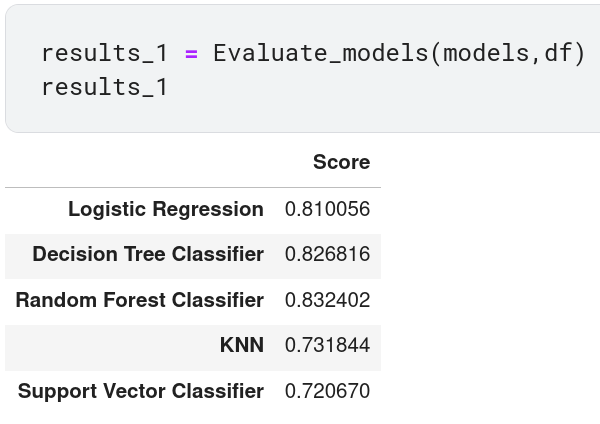
\includegraphics[width=\textwidth]{Figures/results_1.png}
\caption{\label{ml.results}Score dos diferentes modelos de Aprendizado de Máquina.}
\end{figure}

Como pode-se observar, modelos do tipo árvore foram os que melhor desempenho tiveram; seguidos da regressão logística, e finalmente os modelos não-supervisionados apresentaram o pior desempenho.

Após essa observação, aplicamos a técnica de normalização que vimos na seção \ref{feature-Eng}, em nossas features \textsc{Age} e \textsc{Fare} conforme mostrado na Figura \ref{normalized}. O resultado experimental confirma o que estudamos: modelos baseados em árvore e regressão logística são menos sensíveis à normalização. Constatamos na Figura \ref{ml.results2} que de fato, sua pontuação não foi alterada enquanto os modelos não supervisionados apresentaram uma melhora considerável de desempenho. 

\begin{figure}[H]
\centering
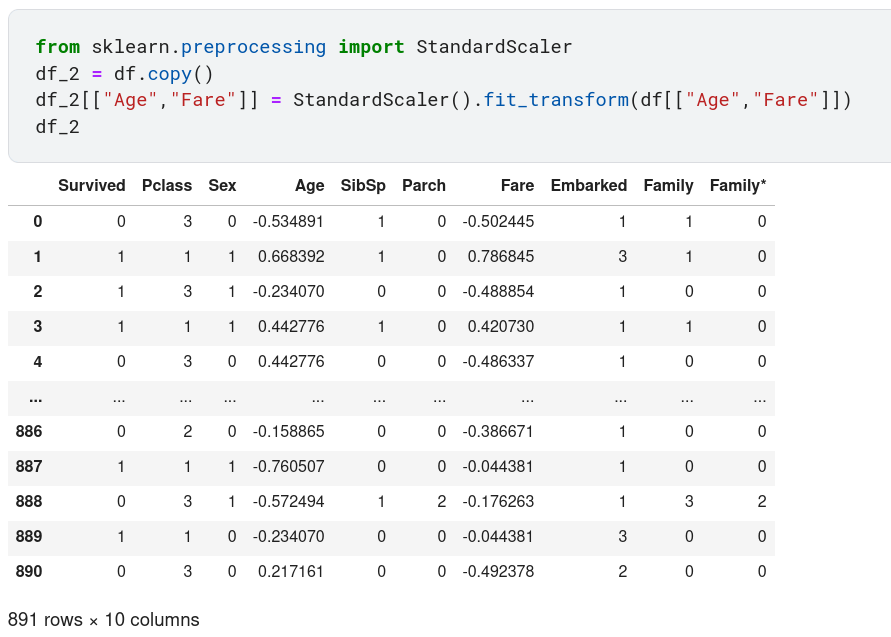
\includegraphics[width=\textwidth]{Figures/normalized.png}
\caption{\label{normalized}Comparação da performance após a normalização de Age e Fare.}
\end{figure}
\begin{figure}[H]
\centering
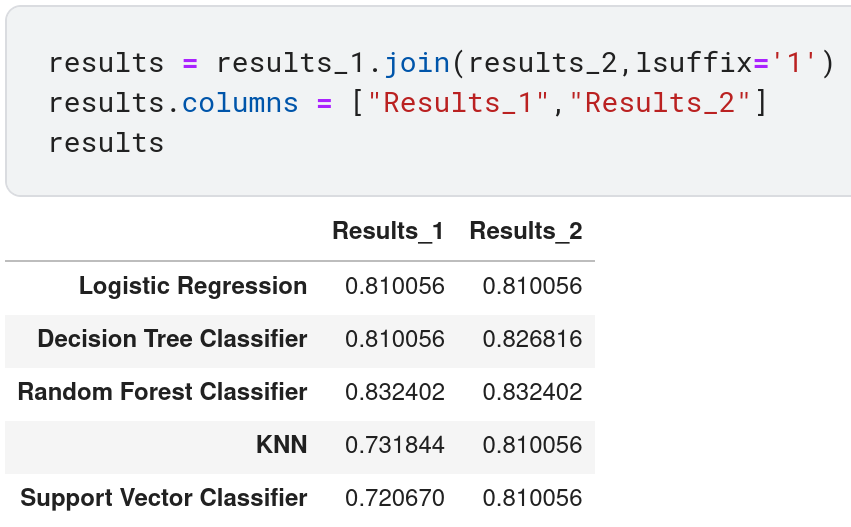
\includegraphics[width=\textwidth]{Figures/results1_2.png}
\caption{\label{ml.results2}Comparação da performance após a normalização de Age e Fare.}
\end{figure}
Assim, concluímos que modelos de arvore funcionaram melhor, especialmente o Random Forest. Também observamos que os tripulantes mais abastados, mulheres, crianças e idosos tiveram mais chance de sobreviver.

\subsection{Data Visualization}
O artigo \cite{BATON} busca definir a ciência de dados e seu modelo de trabalho justamente tendo em vista localizar o papel da visualização de dados dentro desse campo. Concluindo que apesar de pouco reconhecido entre cientistas de dados, o uso da visualização percorre a maior parte das etapas de um projeto de dados. 

Nesse ano de trabalho, a visualização de dados foi usada em diversos momentos das duas etapas anteriores (Análise de Dados e Aprendizado de Máquina), além da apresentação dos resultados. Tanto os gráficos que utilizamos, quanto as tabelas, e até todas as ferramentas, como o próprio conceito de notebook de código estão intimamente entrelaçados com conceitos de apresentação visual de informação, comunicação, arte e fundamentalmente design. 
Assim, um seguimento muito importante desse nosso primeiro ano envolve nos aprofundarmos e mapearmos essa área tão rica e diversa. 

\subsection{Deployment}
\subsubsection{Titanic}
Conforme apresentamos na metodologia, essa etapa final de um projeto de dados envolve transferir a solução construída para o seu ambiente final. Desse modo, para o Titanic, criamos e submetemos o arquivo final com as predições de nosso modelo para cada passageiro presente nos dados do arquivo test.csv. Tais dados são 418 novas entradas para as mesmas 11 colunas de features que o nosso arquivo de treino. Assim, após o treinamento dos modelos, aplicamos o modelo de melhor performance para predizer a sobrevivência desses 418 passageiros. 

Nossa solução obteve o score de aproximadamente 78\% no Kaggle, como mostra a Figura \ref{kaggle.score}. Tal desempenho é compatível com os números encontrados na validação do modelo. Assim, uma vez submetido, podemos permitir que nosso caderno seja acessível ao público. \footnote{https://www.kaggle.com/danielbritodossantos/dbs97-titanic}

\begin{figure}[H]
 \centering
 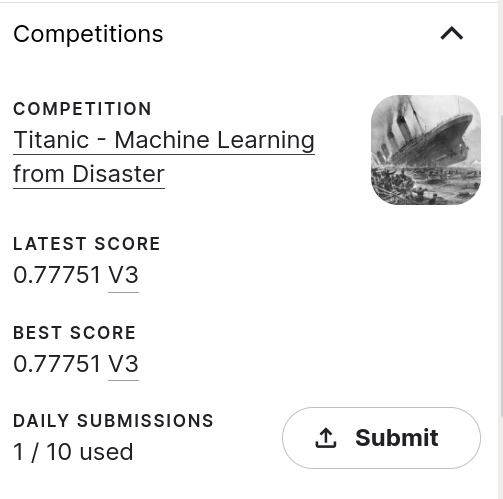
\includegraphics[width=\textwidth]{Figures/Score.png}
 \caption{\label{kaggle.score}Pontuação final no Kaggle.}
\end{figure}
\subsubsection{Aprofundamentos}
Considerando que a entrega final de um projeto de dados pode ser um relatório, o deployment de um modelo ou de uma infra-estrutura computacional, como vimos na seção \ref{principais.conceitos}, nesse ano demonstramos a entrega de um modelo, neste relatório também podemos encontrar aspectos de um relatório de dados.

Entretanto, o deployment de infra estrutura envolve um considerável corpo de conhecimentos. Portanto, nesse ano identificamos os contornos dessa área, esperamos nas próximas etapas desenvolver seus principais conceitos. Tais como redes, aplicações e serviços web, técnicas para armazenagem de funções e modelos treinados, frameworks dentre outras. 

\section{Conclusão}
Assim, podemos afirmar que nosso objetivo principal foi concluído. Uma vez que foi possível percorrer um vasto terreno, compilar diversas técnicas e conceitos, compreender a sua estrutura e como muitas dessas partes dialogam entre si, além de encontramos diversas oportunidades de aprofundamento. 

Assim, concluímos citando Tukey \cite{FoDA} em tradução livre:
\begin{quote}
O futuro da [ciência de dados] pode envolver grande progresso, superar dificuldades reais, e prestar um grande serviço para todos os campos de ciência e tecnologia. Isso vai acontecer? Depende de nós, de nossa vontade de percorrer o caminho difícil dos problemas reais ao invés do caminho suave das premissas irreais, critérios arbitrários e resultados abstratos sem impacto no mundo real. Quem aceita o desafio?
\end{quote}

\section{Perspectiva de continuidade}
A partir da construção dos fundamentos da ciência de dados, identificamos diversas oportunidades de desenvolvimentos futuros, principalmente nas áreas de Data Visualization, Bancos de Dados e Aprendizado de Máquina. Especialmente na possibilidade de nos aprofundarmos em seus corpus de conhecimento e aplicá-los em projetos reais. 
\section{Participação em congressos e trabalhos publicados ou submetidos e outras
atividades acadêmicas e de pesquisa}
O bolsista apresentou a pesquisa em vídeo para o CONFICT 2021\footnote{https://proceedings.science/confict-conpg-2021/papers/ponta-do-iceberg--primeiros-passos-na-ciencia-de-dados} (Figuras \ref{certificado.apresentacao} e \ref{certificado.congressista}) \cite{videoCONFICT}. 

\begin{figure}[h!tbp]
  \centering
  \begin{minipage}[b]{0.7\textwidth}
    \includegraphics[width=\textwidth]{Figures/Galoá Certificate - d4ed9c11-93af-4a39-97c6-0bbe1f7bee10.pdf}
    \caption{\label{certificado.congressista} Certificado de congressista.}
  \end{minipage}
  \hfill
  \begin{minipage}[b]{0.7\textwidth}
    \includegraphics[width=\textwidth]{Figures/Galoá Certificate - f31602c8-c114-485d-a08e-548cd7880738.pdf}
    \caption{\label{certificado.apresentacao} Certificado de apresentação.}
  \end{minipage}
\end{figure}

Também apresentamos os certificados dos minicursos oferecidos pela plataforma Kaggle nas figuras \ref{intro} e \ref{intermediate}.

\begin{figure}[h!tbp]
  \centering
  \begin{minipage}[b]{0.7\textwidth}
    
\includegraphics[width=\textwidth]{Figures/Daniel Brito dos Santos - Intro to Machine Learning.png}
    \caption{\label{intro} Certificado de conclusão do curso introdutório ao aprendizado de máquina.}
  \end{minipage}
  \hfill
  \begin{minipage}[b]{0.7\textwidth}
    
\includegraphics[width=\textwidth]{Figures/Daniel Brito dos Santos - Intermediate Machine Learning.png}
    \caption{\label{intermediate} Certificado de conclusão ao curso intermediário de aprendizado de máquina.}
  \end{minipage}
\end{figure}

\section{Data e assinatura do bolsista (assinatura digitalizada)}


\begin{figure}[H]
 \centering
 
\includegraphics[width=0.4\textwidth]{Figures/Assinatura1.2.png}
 %\caption{\label{kaggle.score}Pontuação final no Kaggle.}
\end{figure}
\center24/01/2022

\section{Data e assinatura do orientador (assinatura digitalizada)}


\begin{figure}[H]
 \centering
 
\includegraphics[width=0.4\textwidth]{Figures/assinatura_annabell.png}
 %\caption{\label{kaggle.score}Pontuação final no Kaggle.}
\end{figure}
\center 28/01/2022

\bibliographystyle{alpha}
\bibliography{bibli}
\end{document}